% /*
%  * ----------------------------------------------------------------------------
%  * "THE BEER-WARE LICENSE" (Revision 42):
%  * <michi.wieland@hotmail.com> and Dumeni Vincenz wrote this file. As long as you retain this notice you
%  * can do whatever you want with this stuff. If we meet some day, and you think
%  * this stuff is worth it, you can buy me a beer in return. Michael Wieland
%  * ----------------------------------------------------------------------------
%  */

\input{../template.tex}

% Dokumentinformationen
\newcommand{\SUBJECT}{Zusammenfassung}
\newcommand{\TITLE}{Microsoft Technologien}

\loadglsentries{glossar}

\input{../front.tex}

\lstset{style=visual-studio-style}

\section{Der Heilige Gral}
\subsection{Reference oder Value}
\begin{itemize}
	\item Man unterscheidet zwischen Referenz- (Klassen) und Value Typen (Structs, Enum und primitive Datentypen)
	\item Bei Referenztypen liegt die Referenz auf dem Stack und das eigentliche Objekt auf dem Heap.
	\item Bei der Parameterübergabe bei Value wird eine Kopie angelegt. Bei Referenztypen wird einfach nur die Referenz auf dem Stack kopiert (nicht aber das Objekt!)
		\item Strings, Arrays und Delegates sind Referenztypen. Es wird immer nur eine Referenz auf dem Stack gespeichert. Bei der Übergabe in Methoden wird nur die Referenz übergeben, nicht so bei Value Typen. Hier wird immer eine Kopie des Wertes übergeben, ausser die Übergabe findet mit dem Schlüsselwort \lstinline|ref| statt.
	\item Ein \lstinline|out| Parameter verhält sich wie ein \lstinline|ref| Parameter, mit dem Unterschied, dass er nicht initialisiert sein muss.
	\item Strings, werden auf dem Heap als \lstinline|char| Arrays alloziert.

\end{itemize}

\begin{figure}[h!]
\centering
\includegraphics[width=0.8\linewidth]{images/reference_value_type}
\caption{Referenz und Value Typen}
\label{fig:valuetypes}
\end{figure}

\clearpage

\subsection{Lamdas}
\begin{itemize}
	\item Lamdas sind anonyme lokale Funktionen welche auch als Argument oder Rückgabewert von Funktionen verwendet werden können.
	\item Lamdas werden in \lstinline|Func<[param_type], [return _type]> myLamda;| gespeichert, wobei der letzte Typ in den spitzen Klammern der Rückgabe Typ ist.
\end{itemize}

\begin{lstlisting}
//verschachtelte Lamda
Func<int,Func<int,string>> curry = a => b => (a + b).ToString();
\end{lstlisting}

\subsection{Delegates, Events}
\begin{itemize}
	\item Der erste Parameter ist bei EventHandler immer immer das \lstinline|this| Objekt!
	\item In einem Event können mehrere Lamda/Funktionen registriert werden (+=)
	\item Wird ein Delegate in einer \lstinline|Func<T>| gespeichert kann das Delegate von überall verwendet werden. Das \lstinline|event| Keyword macht das Delegate privat und generiert public Methoden für die Registrierung und Deregistrierung.
\end{itemize}

\begin{lstlisting}
// defie event handler, where event happens (z.B Schalter)
public event EventHandler<MyEventArgs> MyEventHandler;
// define event args
public MyEventArgs : EventArgs {
	public string Value {get; set; }
}

// register a function to the event
// function is called, when event happens
MyEventHandler += (o, e) => {
	// do anything
}

// Invoke EventHandler
MyEventHandler?.Invoke(this, new MyEventArgs() {
	Value = "test"
});
\end{lstlisting}
\begin{lstlisting}
// without event args
public event Action<bool> MyEvent;
MyEvent?.Invoke(this, true);
// called function with bool param
public void EventHappens(bool state) { this.Light = state; }
MyEvent += Light.EventHappens; // register
\end{lstlisting}

\subsection{Extension Methods}
\begin{itemize}
	\item Eine Extension Method \textbf{und} die Wrapper Klasse müssen \lstinline|static| sein und der erste Parameter der Methode \lstinline|this| als Prefix haben. 
	\item Der erste Parameter definiert die Klasse, welche erweitert wird
\end{itemize}

\begin{lstlisting}
using MyExtensions; // in callee

// simple iterator
public static class MyExtensions {
	public static IEnumerable<T> Ext1<T>(this IEnumerable<T> input) {
		 foreach (T item in input) {
			yield return item;
		}
	}
}
\end{lstlisting}

\clearpage

\subsection{LINQ}
\begin{itemize}
	\item Das Select Statement gibt ein Objekt vom Typ \lstinline|IEnumerable<T>| eines anonymen Types mit den jeweiligen Feldern zurück.
	\item Nützliche Funktionen sind \lstinline|g.Count()|, \lstinline|g.Average(e => e.Amount)|, \lstinline|g.Sum(e => e.Amout)|, \lstinline|x.Min(x => x.Price)|, \lstinline|x.Max(x => x.Price)|
\end{itemize}
\begin{lstlisting}
// extension syntax
var query = myArray
	.Where(e => e.Name.StartsWith("a") && e.Name.EndsWith("b"))
	.GroupBy(e => e.Department)
	.OrderBy(e => e.Name)
	.Select(e => new {
		Name = e.Name,
		Department = (e.Department == null) ? "empty" : e.Department
	})
	.ToList();

// query syntax
var query = from e in myArray
	from d in e.departments
	where e.StartsWith("a")
	group e by e.Name into mygroup [where mygroup.Count() > 3]
	orderby e.Name, d.Name // order by two fields
	select new {
		Name = mygroup.Key,
		Department = d.Name
	};
	
// inner join (==)
var innerJoinQuery =
    from c in categories
    join p in products on c.ID equals p.CategoryID // or compound 'from' over nav prop
    select new { 
	    ProductName = p.Name, 
	    Category = c.Name 
	};
	
// group join (into)
var innerGroupJoinQuery =
    from c in categories
    join p in products on c.ID equals p.CategoryID into prodGroup
    select new { 
	    CategoryName = c.Name, 
	    Products = prodGroup.Count()
	};
	
// left outer join (DefaultIfEmpty() combined with group join)
var leftOuterJoinQuery =
    from c in categories
    join p in products on c.ID equals p.CategoryID into prodGroup
    from item in prodGroup.DefaultIfEmpty(
	    new Product { // set default
		    Name = String.Empty, 
		    CategoryID = 0 
		})
    select new { 
	    CatName = c.Name, 
	    ProdName = item.Name 
	};
\end{lstlisting}

\clearpage

\subsection{Entity Framework}
\begin{itemize}
	\item Über den \lstinline|DbContext| findet die Kommunikation mit der Datenbank statt. Er ist für die Persistierung und Transaktionshandling verantwortlich. Jedes persistente Objekt ist dem DB Kontext zugeornet, was Caching und Tracking von Änderungen erlaubt.
	\item Der Entity Key ist die OO Representation des Primary/Foreign Key. Er wird vom DBContext gesetzt und hat beim Erzeugen den Default Wert seines Types. Sobald die OO Representation in der DB gespeichert wird, wird der Entity Key mit dem Primary Key aus der DB überschrieben.
	\item Für die Sicherstellung der referenziellen Integrität sind die Business Klasse selber zuständig.
	\item Das Entity Framework verwendet standardmässig \textbf{Lazy Loading}. Das bedeutet, dass die Daten erst geladen werden, wenn sie explizit dereferenziert werden. Die Navigation Property muss beim Lazy Loading \lstinline|virtual| sein!
	\item Beim \textbf{Eager Loading} wird das komplette Objekt mit einer \lstinline|Include("A.B")| Anweisung geladen.
\end{itemize}

\begin{lstlisting}
// lazy loading (navigation property needs to be virtual)
public class Blog  {  
	public int BlogId { get; set; }  
	public string Name { get; set; }  
	public string Url { get; set; }  
	public string Tags { get; set; }  
	
	// allows lazy loading
	public virtual ICollection<Post> Posts { get; set; }  
}

// eager loading (load everything at one using Include())
using (var context = new BloggingContext())  {
	var blogs1 = context.Blogs 
		 .Include(b => b.Posts) 
		 .ToList(); 
	
	var blogs2 = context.Blogs 
		 .Include("Posts") 
		 .ToList();
}

// disable lazy loading globally
public BloggingContext() { 
	this.Configuration.LazyLoadingEnabled = false; 
} 
\end{lstlisting}

\clearpage

\subsection{WCF}
\begin{itemize}
	\item Client und Server müssen das gleiche Binding haben. Dieses wird über den Metadata Exchange publiziert (MEX).
	\item Standardmässig werden alle public Properties/Felder eines DTO nach einander serialisiert.
	\item Der Service kann entweder direkt im Code im im XML definiert werden.
	\item Der Client kommuniziert immer über einen Proxy mit dem Service. Der Proxy kann generiert werden (Properties werden in Getter,Setter gewandelt, Listen Typinformationen gehen verloren)
\end{itemize}

\subsubsection{Server}
\begin{lstlisting}[caption=Data Transfer Objects (DTO)]
[DataContract]
[KnownType(typeof(DerivedA))]
[KnownType(typeof(DerivedB))]
public class AModelClass {
	[DataMember]
	public string Name {get; set;}	
}

[DataContract]
public class DerivedA : AModelClass {
	[DataMember]
	public string Name {get; set;}
}

[DataContract]
public class DerivedB : AModelClass, IInterface {
	[DataMember]
	public string Name {get; set;}
}

[DataContract]
public enum MyEnum {
	[EnumMember]
	A,
	[EnumMember]
	Bs
}
\end{lstlisting}
\begin{lstlisting}[caption=Service Interface]
// (may without callback)
[ServiceContract(
	CallbackContract=typeof(IMyCallback),
	SessionMode=SessionMode.Allowed)]
public interface IMyServiceInterface {
	List<AModelClass> Models {
		[OperationalContract[IsOneWay=false]]
		get;
	}
	
	[OperationContract]
	void GetModelById(int id);
	
	[ServiceKnownType(typeof(DerivedB))]
	[OperationContract]
	List<IInterface> getDerivedB();
}

// Callback Interface
public interface IMyCallback {
	[OperationContract(IsOneWay=true)]
	void PassResult(AModelClass model, bool success);
}

\end{lstlisting}
\begin{lstlisting}[caption=Service Implementation]
// Service Implementierung
[ServiceBehaviour(InstanceContextMode=InstanceContextMode.Single)]
public class MyService : IMyServiceInterface {
	private IMyCallback callback = ...;
	private List<AModelClass> models = new List<Models>();
	public List<AModelClass> Models {
		get { return models; }
	}
	
	public void GetModelById(int id) {
		Model model = models.Where(m => m.id = id);
		callback.PassResult(model, true);
	}
	
	public List<IInterface> getDerivedB() {
		return new List<DerivedB>();
	}
}

\end{lstlisting}
\begin{lstlisting}
// Usage (immer die Klasse, nie das Interface!)
ServiceHost myHost = new ServiceHost(typeof([namespace].MyService))
\end{lstlisting}

\begin{lstlisting}[caption=Service Hosting via XML]
<services>
	<service name="[namespace].MyService">
		 <!-- Endpoint: http://localhost:8732/MyService/ -->
		<endpoint address="" binding="basicHttpBinding" contract="[namespace].IMyServiceInterface"/>
		<!-- Endpoint: http://localhost:8732/MyService/mex -->
		<endpoint address="mex" binding="mexHttpBinding"  contract="IMetadataExchange"/> 
		<host>
			<baseAddresses>
				<add baseAddress="http://localhost:8732/MyService/"/>
			</baseAddresses>
		</host>
	</service>
</services>
\end{lstlisting}

\clearpage

\begin{lstlisting}[caption=Service Hosting via Code]
Uri address = new Uri("http://localhost:8732/MyService");
BasicHttpBinding binding = new BasicHttpBinding();

using(ServiceHost host = new ServiceHost(typeof([namespace].MyService), address)) {
	host.AddServiceEndpoint(typeof([namespace].IMyServiceInterface), binding, address);
	host.Open();
	Console.WriteLine("Service ready");
}
\end{lstlisting}

\subsubsection{Client}
\begin{lstlisting}
// name must match with xml name
var factory = new ChannelFactory<IMyServiceInterface>("MyService");
IMyServiceInterface proxy = factory.CreateChannel();
// use
proxy.GetDerivedB();
\end{lstlisting}

\begin{lstlisting}
<xml? version="1.0"?>
<configuration>
	<system.serviceModel>
		<client>
			<endpoint
				address="http://localhost:8732/MyService"
				binding="basicHttpBidning"
				contract="[namespace].IMyServiceInterface"
				name="MyService" />
		</client>
	</system.serviceModel>
</configuration>
\end{lstlisting}

\section{.NET Framework}
\begin{itemize}
	\item Es werden aktuell über 30 Sprachen unterstützt
	\item Der Source Code wird in die Intermediate Language  (IL: Ähnlich wie Assembler, vergleichbar mit Java Bytecode) kompiliert
	\item Alle Sprachen nutzen das selbe Objektmodell und Bibliotheken
	\begin{itemize}
		\item gemeinsamer IL-Zwischencode
		\item gemeinsames Typensystem (CTS)
		\item gemeinsame Runtime (CLR)
		\item gemeinsame Klassenbibliotheken.
		\item Das CLS definiert Einschränkungen an interoperablen Schnittstellen
	\end{itemize}
	\item Der Debugger unterstützt alle Sprachen (auch Cross-Language Debugging möglich)
\end{itemize}
\begin{figure}[h]
\centering
\includegraphics[width=0.6\linewidth]{images/net_framework_architektur}
\caption{.NET Framework Architektur}
\label{fig:netframeworkarchitektur}
\end{figure}

\subsection{CLR: Common Language Runtime}
Die \gls{clr} umfasst mehrere Funtionen wie z.B Just In Time Compilation für die Übersetzung von Intermediate Language Code in Maschinencode. Man versteht unter dem \gls{clr} ein sprachunabhängiges, abstrahiertes Betriebssystem. Es ist verantwortlich für das Memory Management, Class Loading, Garbage Collection, Exceptions, Type Checking, Code Verification des IL-Codes, Threadding
, Debugging und Threading. Die CLR ist mit der Java VM vergleichbar.
\begin{figure}[h]
\centering
\includegraphics[width=0.6\linewidth]{images/common_language_runtime_architektur}
\caption{CLR: Common Language Runtime Architektur}
\label{fig:commonlanguageruntimearchitektur}
\end{figure}

\subsection{CTS: Common Type System}
Das \gls{cts} ist ein einheitliches Typensystem für alle .NET Programmiersprachen. \gls{cts} ist integriert in \gls{clr}. 

\subsection{CLS: Commong Language Specification}
Die \gls{cls} sind allgemeine Regeln für die sprachübergreifende Entwicklung im .NET Framework. CLS kompatible Bibliotheken können in allen .NET Sprachen verwendet werden.

\subsection{MSIL: Microsoft Intermediate Language}
\gls{msil} ist eine \textbf{prozessor-, und sparchunabhängige} Zwischensprache die Assembler ähnelt. 
\begin{enumerate}
	\item Sprachspezifischer Kompilier kompiliert nach MSIL
	\item \gls{jit} Compiler aus dem \gls{clr} kompiliert in nativen plattformabhängigen Code
\end{enumerate}
\paragraph{Vorteile}
\begin{itemize}
	\item Portabilität
	\item Typsicherheit: Beim Laden des Codes können Typensicherheits und Security Checks durchgeführt werden.
\end{itemize}
\paragraph{Nachteile}
\begin{itemize}
	\item Performance (kann verbessert werden, wenn JIT Compiler prozessorabhängige Hardwarebeschleunigung nutzt.)
\end{itemize}

\begin{figure}[h]
\centering
\includegraphics[width=0.5\linewidth]{images/msil_compilation}
\caption{MSIL Kompilierung}
\label{fig:msilcompilation}
\end{figure}

\subsection{JIT: Just in Time Compilation}
Bei der JIT Kompilierung wird die aufgerufene Methode vor dem Methodenaufruf kompiliert und der IL-Code durch nativen Code ersetzt.

\subsection{Assembly / Komponenten}
\begin{figure}[h!]
\centering
\includegraphics[width=0.7\linewidth]{images/assembly}
\caption{Assembly Übersicht}
\label{fig:assembly}
\end{figure}

Ein Assembly kann mit einem JAR File verglichen werden. Ein Assembly enthält MSIL-Code, Typ und Assembly Metadaten, Manifest mit strong names (Version/Author) und Referenzen auf andere Assemblies. Ein Assembly \textbf{kann aus mehreren Modulen bestehen}, \textbf{standardmässig} enthält ein Assembly aber \textbf{genau ein Modul}. Assemblies können nicht geschachtelt werden!
\begin{description}
	\item[Private Assembly] Private Assembly werden über einen Dateipfad referenziert und sind ansonsten nirgends registriert. Sie werden meist nur von einer Applikation genutzt.
	\item[Shared Assembly] Shared Assemblies verfügen über einen Strong Name (eindeutige Bezeichnung: Bez, Version, Culture, Public Key) und liegen im Global Assembly Cache (GAC). Ein Shared Assembly steht allen Applikationen zur Verfügung. Es sollte nicht zu viele Versionen im GAC registriert werden. (DLL Hell). Für die registriert wird das Command Line Tool \lstinline|gacutil.exe| verwendet.
\end{description}

\subsubsection{Module}
Die Kompilation erzeugt ein Modul mit Code / \gls{msil} und Metadaten. Die Metadaten beschreiben alle Aspekte des Codes ausser der Programmlogik. (Klassen, Methoden und Feld Definitonen) Diese Metadaten können mit Reflektion abgefragt werden.

\subsubsection{References}
Referenzen zeigen auf eine externe Library. \\
Referenzen werden beim CSC mittels \lstinline|csc /target:exe /r:MyDLL.dll Program.cs| eingefügt.


\clearpage

\subsection{Kompilierung}
Zur Kompilierung wird der \gls{csc} verwendet.  
\begin{lstlisting}
// Create Executable: ClassA.exe
csc.exe /target:exe ClassA.cs

// Create Lib: ClassA.dll
csc.exe /target:library ClassA.cs

// Create Executable, referencing a Lib
csc.exe /target:exe
		/out:Programm.exe
		/r:ClassA.dll // or /r:System.Windows.Forms.dll (GAC)
		ClassB.cs ClassC.cs
// Ergibt = Program.exe
\end{lstlisting}

\subsection{Garbage Collection}
Der Garbage Collector löscht Objekte auf dem Heap, die nicht mehr über eine Root-Referenz referenziert werden. (Mark and Sweep) Wie in Java weiss man nicht wenn der GC aufgerufen wird (\textbf{nicht deterministisch}). Er kann aber mit der Methode GC.Collect() manuell aufgerufen werden. Der Ablauf ist immer gleich:
\begin{enumerate}
	\item Alle Objekte als Garbage betrachten
	\item Alle reachable Objekte markieren
	\item Alle nicht markierten Objete freigeben
	\item Speicher kompaktieren
\end{enumerate}

Die Garbage Collection started, sobald eine dieser Bedingungen wahr ist
\begin{itemize}
	\item System hat zu wenig Arbeitsspeicher
	\item Allozierte Objekte im Heap übersteigen einen Schwellwert
	\item GC.Collect Methode wird aufgerufen.
\end{itemize}

\paragraph{Root Referenzen}
Root-Referenzen sind statische Felder und aktive lokale Variablen auf dem Stack.

\subsubsection{Generationen}
Objekte werden in drei Generationen aufgeteilt: Zuerst werden die Objekte der 0ten Generation abgeräumt.
\begin{itemize}
	\item Generation 0: Objekte wurden seit dem letzten GC Durchlauf neu erstellt (z.B lokale Variablen)
	\item Generation 1: Objekte die einen GC Durchlauf überlebt haben (z.B Members)
	\item Generation 2: Objekte die mehr als einen GC Durchlauf überlebt haben.
\end{itemize}

\subsubsection{Deterministic Finalization} Objekte sollten wenn nötig mit dem Interface \lstinline|IDisposable| und der \lstinline|void Dispose()| Methode finalisiert werden und nur wenn nötig mit einem Destruktor. Man spricht von Deterministic Finalization, wenn der Programmierer für die Freigabe der unmanaged Ressourcen zuständig ist und diese explizit über \lstinline|Dispose()| freigibt. Dazu muss die \lstinline|Dispose()| Methode überschrieben werden. Mit \lstinline|using| wird der Aufrufe von \lstinline|Dispose()| implizit sichergestellt. Deterministic Finalization sollte bei allen I/O Klassen verwendet werden.
\begin{itemize}
	\item Dateisystem Zugriffe
	\item Netzwerk Kommunikation
	\item Datenbank Anbindung
\end{itemize}

\begin{lstlisting}
public class DataAccess : IDisposable {
	private DbConnection connection;
	public DataAccess() { 
		connection = new SqlConnection();
	}
	
	~DataAccess() {
		// backup
		connection.Dispose(); 
	}
	
	public void Dispose() {
		// supress GC, as we just want to call dispose
		System.GC.SuppressFinalize(this);
		connection.Dispose();
		// Call base.Dispose(); if necessary
	}
}

using (DataAccess dataAccess = new DataAccess()) {
	// work with dataAccess
}
\end{lstlisting}

\subsubsection{Finalizer} Der Gebrauch von herkömmlichen Finalizer ist nicht deterministisch (man weiss nicht wann der GC aufgerufen wird). Der Garbage Collector arbeitet viel effizienter wenn kein Destruktor/Finalizer vorhanden ist. Einflüsse auf den GC Aufruf sind folgende:
\begin{itemize}
	\item Gerade verfügbarem Speicher
	\item Generation des aktuellen Objektes
	\item Reihenfolge in der Finalization Queue
	\item Manuell oder automatisch getriggert
	\item Kann auch abhängig von der .NET Runtime Version sein
\end{itemize}

\subsubsection{Object Pinning} Der GC kompaktiert Speicher bei Bedarf. Mit dem Keyword \lstinline|fixed| kann dies unterbunden werden. (schlechte Performance)

\subsubsection{Weak References} Wird eine strong Referenz (default) auf null gesetzt, wird es irgendwann vom GC abgeräumt. Auf das null objekt kann nicht mehr zugegriffen werden. Mit Weak Refenzen kann man immer noch auf das Objekt zugreifen, bis es vom GC abgeräumt wird. Mit der Methode \lstinline|TryGetTarget(out sr)| kann man auf das alte Objekt zugreifen und dieses wiederherstellen. Wurde das Objekt abgeräumt, muss es neu erstellt werden.

\subsubsection{Memory Leaks} Memory Leaks entstehen, wenn z.B ein Event Listener nicht abgeräumt wird. Objekte welche aus einer anonymen Methode oder Lamda Ausdruck innerhalb eines Event Listener noch referenziert werden, werden nicht abgeräumt. Gleiches gilt für alle IDisposable Objekte, bei denen \lstinline|Dispose()| nicht aufgerufen wurde. (z.B DB Connection)

\begin{lstlisting}
// interface
public interface IDisposable {
	void Dispose();
}
	
// deterministic finalization
public class DataAccess : IDisposable {
		private DbConnection connection;
		public DataAccess() {
			connection = new SQLConnection();
		}
	
	~DataAccess() {
		connection.Dispose();
	}
	
	public void Dispose() {
		System.GC.SuppressFinalize(this);
		connection.Dispose();
	}
}

class MyClass {
	// call disposal
	DataAccess dataAccess = new DataAccess() ;
	dataAccess.Dispose();
	
	// implicit Disposal call with using
	// Multiple usings possible
	// syntactic sugar, compiles to try-finally with Dispose call
	using (DataAccess dataAccess = new DataAccess())
	using (SQLParser parser = new SQLParser()) {
		..
	}
	
	// or with same type
	using (DataAccess da1 = new DataAccess(), DataAccess da2 = new DataAccess()) {
		..
	}
}
\end{lstlisting}


\section{Visual Studio 15}
\subsection{Solution}
Eine Solution besteht aus mehreren Projekten.

\subsection{Umbenennen}
Folgende Objekte müssen manuell umbenannt werden
\begin{itemize}
	\item Ordner in der das Projekt liegt 
	\begin{enumerate}
		\item Manuelle Anpassung des Ordner Names in File-System
		\item  Manuelles Anpassen der *.sln-Datei
	\end{enumerate}
	\item Name des Assemblies
	\begin{itemize}
		\item Rechts-Klick auf Projekt > Properties > Application > Assembly name
	\end{itemize}
	\item Name des Default Namespaces (wird bei neuen Classen verwendet)
	\begin{itemize}
		\item Rechts-Klick auf Projekt > Properties > Application > Default namespace
	\end{itemize}
\end{itemize}

\subsection{Ordnerstruktur}
Jeder Projektordner enthält folgende zwei Verzeichnisse
\begin{description}
	\item[bin\textbackslash<BuildKonfiguration>] \hfill \\
	Beinhaltet das fertige, gelinkte Kompilat
	\item[obj\textbackslash<BuildKonfiguration>] \hfill \\
	Beihaltet Files welche während der Kompilierung erzeugt werden und für die Erstellung eines Assemblies nötig sind.
\end{description}


\section{C\# Grundlagen}
\subsection{Unterschiede zu Java}
\begin{itemize}
	\item Es gibt Structs, welche wie Klassen sind (jedoch Wertetypen)
	\item Es gibt Properties (spez. Getter und Setter) und Indexer (erweiterter Array Zugriff)
	\item Andere Syntax bei den Konstruktoren
	\item Es gibt Operator Overloading
	\item Parameterübergabe kann explizit by value oder by reference sein (auch für Wertetypen)
	\item Es gibt partielle Klassen und Methoden für Generatoren
	\item Es heisst \lstinline|NullReferenceException| und nicht \lstinline|NullPointerException|
	\item Es heisst \lstinline|base| und nicht \lstinline|super|
	\item Konstruktorparameter können direkt dem Parent übergeben werden. (\lstinline|public Derived(int x) : base(x) { .. }|)
\end{itemize}

\subsection{Naming Conventions}
\begin{table}[h]
	\centering
	\begin{tabu} to \linewidth {l l l}
		\toprule 
		Element & Casing  & Beispiel \\
		\midrule
		Namespace & PascalCase & System.Collections.Generic \\
		Klasse, Struct & PascalCase & BackColor \\
		Interface & PascalCase & IComparable\\
		Enum & PascalCase & Color\\
		Delegates & PascalCase & Action / Func\\
		Methoden & PascalCase & GetDataRow, UpdateOrder\\
		Felder & CamelCase & name, orderId \\
		Properties & PascalCase & OrderId \\
		Events & PascalCase & MouseClick \\
		\bottomrule
	\end{tabu} 
	\caption{Naming Conventions}
\end{table}

\subsection{Sichtbarkeiten}
\begin{itemize}
	\item Abgeleitete Klasse/Interfaces dürfen nicht die grössere Sichtbarkeit als ihren Basistyp haben (z.B Parent ''internal'' und Sub ''public'')
	\item Member Typen müssen mindestens gleich sichtbar wie der Typ selbst sein
	\item Standad Sichtbarkeit ist \lstinline|internal|
	\item Interface Member dürfen keine Angaben zur Sichtbarkeit haben.
\end{itemize}
\begin{table}[h]
	\centering
	\begin{tabu} to \linewidth {l l}
		\toprule 
		Attribut & Beschreibung \\
		\midrule
		public & Überall sichtbar \\
		private & Innerhalb des jeweiligen Typen sichtbar (Klasse/Struct) \\
		protected & Innerhalb des jeweiligen Typen oder abgeleiteten Klasse sichtbar (Klasse/Struct) \\
		internal & Innerhalb des jeweiligen Assemblies sichtbar \\
		protected internal & Kombination aus internal und protected \\
		\bottomrule
	\end{tabu} 
	\caption{Sichtbarkeiten}
\end{table}

\begin{table}[h]
	\centering
	\begin{tabu} to \linewidth {l l l X}
		\toprule 
		Typ & Sichtbarkeit & Member (default) & Member (zulässig)\\
		\midrule
		class & public, internal(default) & private & public, protected, internal, private, protected internal \\
		struct & public, internal(default) & private & public, internal, private \\	
		enum & public, internal(default) & public & - \\
		interface & public, internal(default) & public & - \\
		delegate & public, internal(default) & - & - \\
		\bottomrule
	\end{tabu} 
	\caption{Standard Sichtbarkeiten von Typen}
\end{table}

\newpage

\subsection{Operatoren}
\begin{figure}[h!]
\centering
\includegraphics[width=\linewidth]{images/operator_prezedenz}
\caption{Operatoren Präzedenz}
\label{fig:operatorprezedenz}
\end{figure}

\clearpage

\subsection{Pre-, Post-Inkrmenet}
\begin{lstlisting}
// post increment
int a = 1;
int b = a++; // a=2, b=1

// pre increment
a = 1;
b = ++a; // a=2, b=2
\end{lstlisting}

\subsection{Statements}
\subsubsection{If Else If Else}
\begin{lstlisting}
if () {
} else if () {
} else {}
\end{lstlisting}

\subsubsection{Switch Case}
\begin{lstlisting}
switch() {
case:
case: break;
}
\end{lstlisting}

\subsubsection{Loops}
\begin{lstlisting}
while() {}
do {} while ();
for (int = 1; i <= myList.Count(); i++) {}
foreach(int x in y);
\end{lstlisting}

\subsubsection{Kommentare}
\begin{lstlisting}
// Single Line Comment
/* Multiline Comment */
/// Dokumentation
\end{lstlisting}

\clearpage

\subsection{Datentypen}
Numerische Datentypen können einen der folgenden Literale haben
\begin{figure}[h!]
\centering
\includegraphics[width=0.8\linewidth]{images/primitive_types}
\caption{Primitive Typen}
\label{fig:primitivetypes}
\end{figure}

\begin{itemize}
	\item u/U: unsigned (signed Variablen können nur mit einem cast einer unsigned Variablen zugewiesen werden)
	\item l/L: long
	\item f/F: float
\end{itemize}
\begin{figure}[h!]
\centering
\includegraphics[width=0.8\linewidth]{images/datatypes}
\caption{Datentypen}
\label{fig:datatypes}
\end{figure}

\begin{figure}[h!]
\centering
\includegraphics[width=\linewidth]{images/default_values}
\caption{Default Values}
\label{fig:defaultvalues}
\end{figure}

\newpage

\subsubsection{Casts}
\begin{figure}[h!]
\centering
\includegraphics[width=\linewidth]{images/casts}
\caption{Casts}
\label{fig:casts}
\end{figure}

\clearpage

\subsubsection{Reference Types / Referenztypen}
\begin{itemize}
	\item Sind auf dem Heap gespeichert, wobei die Variable an sich auf dem Stack liegt
	\item Die Referenzen werden automatisch vom Garbage Collector aufgeräumt
	\item Wird ein Reference Type einer Methode übergeben, wird die Objekt referenz kopiert. (sofern nicht \lstinline|ref|)
\end{itemize}

\subsubsection{Value Types / Werttypen}
\begin{itemize}
	\item Sind auf dem Stack gespeichert
	\item Primitive Datentypen, Struct und System.Enum
	\item Wird eine Value Type Variable einer weiteren Value Type Variable zugewiesen, wird der Wert kopiert. Gleiches gilt für die Methodenparameter by Value.
\end{itemize}

\begin{figure}[ht!]
	\centering
	\begin{minipage}[t]{0.4\textwidth}
		\centering
		\includegraphics[width=0.8\linewidth]{images/reference_types}
		\caption{Referenztypen}
		\label{fig:searchtreeinsert1}
	\end{minipage}
	\begin{minipage}[t]{0.4\textwidth}
		\centering
		\includegraphics[width=0.8\linewidth]{images/value_types}
		\caption{Wertetypen}
		\label{fig:searchtreeinsert2}
	\end{minipage}
\end{figure}

\clearpage

\subsection{Nullable Types}
\begin{itemize}
	\item Der ? Operator erlaubt es Null Werte einem Wertetyp zuzuweisen. Der Typ ist dann \lstinline|Nullable<T>|
	\item Arithmetisch Ausdrücke mit Null ergeben immer \lstinline|null|
	\item Vergleiche mit Null sind immer \lstinline|false|. Ausnahme \lstinline|null == null|
	\item Der ?? Operator erlaubt es einen Default Wert anzugeben, falls die Variable leer ist
\end{itemize}
\begin{lstlisting}
int a = 0;
bool b = false;
int? c = 10;
int? d = null;
int? e = null;

c + a // 10, typof int?
a + null // null
a < c //true
a + null < c // false
a > null // false
(a + c - e) * 9898 + 1000 // null
d // null
d == d // true
c ?? 1000 // 10
d ?? 1000 // 1000

-------------------------------------

int a = 1;
int? b = 2;
int? c = null;

a+1; // 2
a+b; // 3
a+c; // null
a < b; // True
a < c; // False
a + null; // null
a + null < b; // False
a + null < c; // False
a + null == c; // True
\end{lstlisting}

\clearpage

\subsection{Boxing / Unboxing}
Beim Boxing werden Value Typen implizit in Referenztypen konvertiert. Das Unboxing erfolgt immer explizit. 
\begin{lstlisting}
// boxing
int i = 123;
object o = i;

// unboxing
o = 123;
i = (int) o;
\end{lstlisting}

\begin{figure}[h!]
\centering
\includegraphics[width=0.4\linewidth]{images/boxing}
\caption{Boxing}
\label{fig:boxing}
\end{figure}



\subsection{Object}
\begin{itemize}
	\item \lstinline|object| ist ein Alias für \lstinline|System.Object|
\end{itemize}

\subsection{String}
\begin{itemize}
	\item \lstinline|string| ist ein Alias für \lstinline|System.String|
	\item String ist ein Reference Type
	\item Wie in Java ist ein String nicht modifizierbar
	\item Mit dem \lstinline|@| vor dem String Literal kann der String Sonderzeichen enthalten, die nicht escaped werden müssen.
\end{itemize}
\begin{lstlisting}
// Escape: The "File" can be \t found at \\server\share
@"The ""File"" can be \t found at \\server\share"

// Formatieren
string f = string.Format("A={0} and B={1}", a, b);

// Kopieren
string s2 = string.Copy(s1);

// Vergleichen
s1.Equals(s2) // Inhalt wird verglichen, nicht die Referenz
s1 == s2 // Inhalt wird verglichen, nicht die Referenz
s1.CompareTo(s2); // -1, 0, +1 
string.ReferenceEquals(s1, s2); // Achtung: String Pooling, nach Copy = False
\end{lstlisting}

\clearpage

\subsection{Arrays}
\begin{lstlisting}
int[] array1 = new int[5]; // deklaration value type
int[] array2 = {1,2,3,4,5}; // deklaration & wertedefinition
int[] array3 = int[] {1,2,3,4,5,6}; // vereinfachte syntax ohne typ
int[] array4 = {1,2,3,4,5,6}; // vereinfachte syntax ohne Typ / new
object[] array5 = new object[5]; // deklaration ref type
array1.Length // Get Length

// Blockmatritzen (Speichereffizienter und schneller im Zugriff)
int[,] multiDim1 = new int[2,3];
int[,] multiDim2 = { {1,2,3} , {4,5,6} };

// Jagged Arrays
int[][] jaggedArray = new int[6][];
jaggedArray[0] = new int[4] { 1, 2, 3, 4 }
\end{lstlisting}

Ablage von Arrays nach Jagged- Blockmatrizen-Prinzip:
\begin{figure}[h!]
\centering
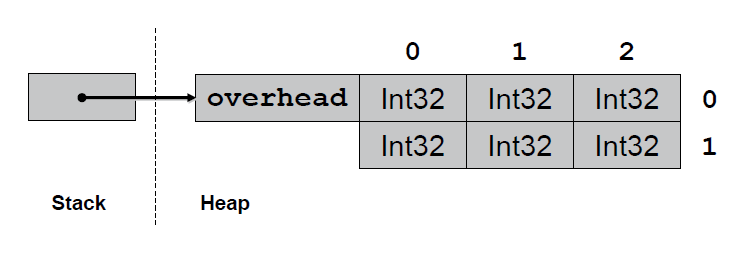
\includegraphics[width=0.7\linewidth]{images/matrizenarray}
\caption{Blockmatrizen}
\label{fig:Blockmatrizen}
\end{figure}

\begin{figure}[h!]
\centering
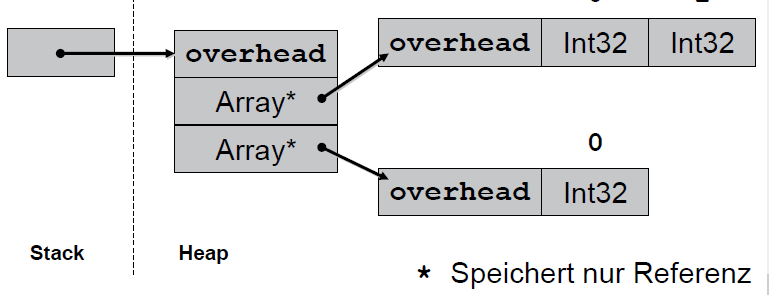
\includegraphics[width=0.7\linewidth]{images/jaggedarray.png}
\caption{Jacked}
\label{fig:Jacked}
\end{figure}

\subsection{Indexer}
Ein Indexer erlaubt einfachen Zugriff auf ein Array. Er wird mit dem Keyword \lstinline|this| erstellt.
\begin{lstlisting}
class BookList {
	private string[,] books ={{},{},{}};

	public string this[int i1, int i2] {
		get { return books[i1, i2]; }
		set { books[i1, i2] = value;  } 
	}
}

// access
bookList[0, 0]
\end{lstlisting}

\subsection{List}
\begin{lstlisting}
var myList = new List<int>() { 1, 2, 3, 4, 5 }; // using System.Collections.Generic;
myList.Count(); // Or Property when var x = myList.Count;
myList.Add(6);
myList.Remove(4);
myList.Contains(6); // True
myList.ForEach(n => Console.WriteLine(n)); // 1,2,3,5,6
myList.Clear();
myList[4];
myList.IndexOf(4);
\end{lstlisting}


\subsection{Namespaces}
Namespaces entspricht dem Package in Java und lässt den Code hierarchisch strukturieren. Ein Namespace ist nicht an die physische Struktur gebunden. (in Java schon)
\begin{lstlisting}
namespace A {
	using C;
	public class A : Base {
		C.externMethod();
	}
}
\end{lstlisting}

\section{Variablen und Properties}
\subsection{Konstanten}
Der Wert einer Konstante muss zur Compilezeit verfügbar sein.
\begin{lstlisting}
const long size = int.MaxValue;
\end{lstlisting}

\subsection{ReadOnly}
Readonly Felder müssen in der Deklaration oder im Konstruktor initialisert werden. Readly Variablen sind äquivalent mit Java final Felder
\begin{lstlisting}
	readonly DateTime date1 = DateTime.Now;
	
	class Test {
		private readonly int myProp;
		public int MyProp {
			get { return myProp; }
		}
		
		public Test() {
			myProp = 42;
		}
	}
\end{lstlisting}

\subsection{Properties}
Eine Property ist ein Wrapper um Getter und Setter. Get und Set können einzeln weggelassen werden. (read-only, write-only) Bei Set besteht zudem die Möglichkeit das Flag private zu setzen. 
\begin{lstlisting}
	// Backing Field
	private int lenght;
	
	public int Length {
		get { return length; }
		// private is optional
		private set { length = value; } 
	}
	
	MyClass mc = new MyClass();
	mc.Length = 12;
	int length= mc.Length;
	
\end{lstlisting}

\subsubsection{Auto Properties}
Bei Auto Properties wird das Backing Field sowie die zugehörigen Getter und Setter automatisch generiert.
\begin{lstlisting}
	// Auto Property: Backing field is auto generated
	public int LengthAuto { get; set; }
	public int LengthInitializes {get; /* set; */ } = 5;
\end{lstlisting}

\subsubsection{Properties direkt initialisieren}
Properties können bei der Objekt erstellung direkt initialisiert werden. 
\begin{lstlisting}
	MyClass mc = new MyClass() {
		Length = 1;
		Width = 2;
	}
\end{lstlisting}

\section{Methoden}
\subsection{Overloading}
Methoden können \textbf{überladen} werden. (Unterschiedliche Anzahl Parameter, Unterschiedliche Typen, Unterschiedliche Parametertypen (ref/out) aber immer gleicher Name)
\begin{lstlisting}
public static void Foo(int x);
public static void Foo(doubly y);
public static void Foo(int x, int y);
public static void Foo(params int[] x); // params array = normales array

// sollte man nicht machen. Design Problem!
public static void Foo(int ref x);
public static void Foo(int out x);
\end{lstlisting}

\subsection{Call by value}
Es wird eine Kopie des Stack Inhalts übergeben
\begin{lstlisting}
void IncVal(int x){}
int val = 3; 
IncVal(val); // pass copy
\end{lstlisting}

\subsection{Call by reference}
Adresse der Variable wird übergeben. Mit dem \lstinline|ref| Keyword können auch Werttypen als Referenz übergeben werden.
\begin{lstlisting}
void IncRef(ref int x) {}
int value=3;
IncRef(ref value); // pass reference, value must be initialized (default param value possible too)
\end{lstlisting}

\subsection{Out Parameter}
Das \lstinline|out| Keyword erlaubt es Werte by Reference zu übergeben. Es funktioniert wie das \lstinline|ref| Keyword, mit dem Unterschied, dass die Variable nicht im Vorhinein initialisiert werden muss. Das \lstinline|out| Keyword muss beim Aufrufer und bei der Methode deklariert werden.
\begin{lstlisting}
static void Init(out int a) {
	a = 10;
}

// usage
int value;
Init(out value); 
// value is now 10 
\end{lstlisting}

\subsection{Params Array}
Erlaubt beliebig viele Parameter. Das params Array muss am Ende der Deklaration stehen.
\begin{lstlisting}
void Sum(out int sum, params int[] values) { .. }
Sum(out sum2, 1,2,3,4);
\end{lstlisting}

\subsection{Optionale Parameter (Default Values)}
Erlaubt ermöglicht Zuweisung eines Default Values. Die Optionalen Parameter dürfen erst am Schluss deklariert werden. Default Werte können bei \lstinline|out| und \lstinline|ref| Parameter nicht verwendet werden.
\begin{lstlisting}
private void Sort(
	int[] array,            // Erforderlich
	int from = 0,           // Optional
	int to = -1,            // Optional
	bool ascending = true,  // Optional
	bool ignoreCase = false // Optional
	){ .. }
\end{lstlisting}

\subsection{Named Parameter}
Optionale Parameter können über den Namen identifiziert und übergeben werden.
\begin{lstlisting}
Sort(a, ignoreCase: true, from: 3);
\end{lstlisting}

\subsection{Virtual}
Bei C\# wird alles statisch gebunden. Mit dem Keyword \lstinline|virtual|, wird dynamisch gebunden. Bei einer virtuellen Methode wird deshalb die überschriebene Methode in der Subklasse aufgerufen. Virtual kann nicht mit folgenden Keywords verwendet werden.
\begin{itemize}
	\item \lstinline|static|
	\item \lstinline|abstract| (implizit virtual)
	\item \lstinline|override| (implizit virtual)
\end{itemize} 

\subsection{Override}
Mit dem Keyword \lstinline|override| können \lstinline|virtual| Methoden überschrieben werden. Die Signatur muss dabei identisch sein. Man spricht von dynamischem Binding.


\begin{lstlisting}
public class Base {
	public virtual void Invoke() {
		Console.WriteLine("Base");
	}
}
public class Derived : Base {
	public override void Invoke() {
		Console.WriteLine("Derived");
	}
}

Base a = new Base();
Base b = new Derived();
Derived c = new Derived();

a.Invoke(); // base
b.Invoke(); // derived
c.Invoke(); // derived
\end{lstlisting}

\clearpage

\subsection{New}
Mit \lstinline|new| weiss der Compiler, dass der Member bewusst überdeckt wurde. Man spricht von \textbf{statischem Binding}. Es wird immer die Methode des statischen Typs ausgeführt. New kann \textbf{nicht} mit \lstinline|override| verwendet werden, jedoch mit \lstinline|virtual|.
\begin{lstlisting} 
public class Base {
	public void Invoke() {
		Console.WriteLine("Base");
	}
}
public class Derived : Base {
	public new void Invoke() {
		Console.WriteLine("Derived");
	}
}

Base a = new Base();
Base b = new Derived();
Derived c = new Derived();

a.Invoke(); // base
b.Invoke(); // base
c.Invoke(); // derived
\end{lstlisting}

\subsection{Sealed}
Mit \lstinline|sealed| weiss der Compiler, dass die Methode (kein Overriding) oder Klasse (keine Vererbung) nicht mehr verändert wird. Es ist das Pendant zum Java \lstinline|final|.
\begin{lstlisting} 
public sealed void MyFunc()
\end{lstlisting}

\section{Klassen, Structs}
\subsection{Klassen}
\begin{itemize}
	\item Klassen sind Refenztypen die auf dem Heap abgelegt werden
	\item Klassen können ineinander verschachtelt sein. Die Inner Class hat dabei Zugriff auf alle Member der Outer Class. Die Inner Class wird mit \lstinline|OuterClass.InnerClass inner = new OuterClass.InnerClass();| initialisiert.
	\item Klassen können statisch sein. Statische Klassen können nicht abgeleitet werden. Es gibt auch statische Imports \lstinline|using static System.Math|
	\item Hat immer einen Default Konstruktor, sofern nicht ein anderer definiert wurde.
	\item Links steht immer der statische Typ und rechts der dynamische
\end{itemize}
\begin{lstlisting}
public class MyClass : Base

// check if class is instance of
Sub s = new Sub();
if (s is Base) {}
\end{lstlisting}

\subsubsection{Type Casts}
Type Casts können mit den runden Klammern oder mit dem Keyword \lstinline|as| gemacht werden. \lstinline|as| liefert \lstinline|null| zurück, wenn nicht gecasted werden kann (anstatt eine Exception zu werfen). 
\begin{lstlisting}
// type cast
Base b = new Sub();
Sub s = (Sub) b; // could throw InvalidCastException

// cast with 'as'
Sub s = b as Sub; // returns null if cast not possible

// check if class is instance of
Sub s = new Sub();
if (s is Base) {}
\end{lstlisting}

\subsubsection{Operatoren Überladen}
\begin{lstlisting}
public class Vector{
	private int x, y;
	
	public Vector(int x, int y) {};
	
	// must be static
	public static Vector operator + (Vector a, Vector b) {
		return new Vector(a.x + b.x, a.y + b.y);
	}						
}
\end{lstlisting}



\subsubsection{Methoden überschreiben}
Methoden können in einer abgeleitete Klasse überschrieben werden. Dabei gilt folgende Ausfürhungsreienfolge je nach Instatierungvariante.
\begin{lstlisting}
class Vehicle { 
 public virtual void WhoAreYou() { 
   Console.WriteLine("Vehicle"); 
 } 
} 
class Car : Vehicle { 
  public override void WhoAreYou() { 
    base.WhoAreYou(); Console.WriteLine("Car"); 
  } 
} 
class SportCar : Car { 
  public new void WhoAreYou() { 
    base.WhoAreYou(); Console.WriteLine("SportCar"); 
  } 
}

//weil ein Objekt von Car instanziert wird nur die Methode von Vehicle und Car aufgerufen.
Car c1 = new SportCar(); 
c1.WhoAreYou();
//im gegensatz dazu wird bei c2 die Methode bei Vehicle, Car, und Sportcar aufgerufen
SportCar c2 = new SportCar(); 
c2.WhoAreYou();

\end{lstlisting}

\subsubsection{Partial Class}
Das \lstinline|partial| Keyword erlaubt die Definition in mehreren Files. Es sind auch partielle Methoden möglich
\begin{lstlisting}
partial class MyClass { public void Test1() { .. } }
partial class MyClass { public void Test2() { .. } }

MyClass mc = new MyClass();
\end{lstlisting}

\subsection{Abstrakte Klassen}
\begin{itemize}
	\item Abstrakte Klassen können nicht direkt instanziert werden. 
	\item Alle abstrakte Member müssen implementiert sein (\lstinline|override|)
\end{itemize}
\begin{lstlisting}
abstract class Sequence {
	public abstract void Add(object x); // implicit virtual, no implementation
	public abstract string Name { get; }; // property
	public abstract object this[int i]{ get; set; }; // indexer
	public abstract event EventHandler OnAdd; // Event;
	
	public override string ToString() {return Name; }; 
}

class List : Sequence {
	public override void Add(object x)
}
\end{lstlisting}

\subsection{Sealed Klassen}
Von versiegelten ''\lstinline|sealed|'' Klassen kann nicht abgeleitet werden. Es verhält sich also wie das \lstinline|final| bei Java.
\begin{lstlisting}
sealed class Sequence {
	// members can also be sealed:
	public sealed void X();
}

class List : Sequence {} // Compiler error

class Sequence {
	// cannot be overwritten, but 'new' is possible
	public sealed void X();
}

\end{lstlisting}

\subsection{Statische Klassen}
Statische Klassen sind implizit \lstinline|sealed|. Sie dürfen nur statische Member enthalten und können nicht instanziiert werden.
\begin{lstlisting}
static class MyMath {
	public const double Pi = 3.14159;
	public static double Sin(Double x) { .. }
}
\end{lstlisting}
\clearpage

\subsection{Structs}
\begin{itemize}
	\item Structs sind Valuetypen die auf Stack liegen
	\item Structs sind Valuetype und können deshalb nie \lstinline[]|null| sein.
	\item Structs können weder vererben noch erben. (Interfaces sind aber möglich)
	\item Structs benötigen weniger Speicherplatz wie Klassen
	\item Es gibt keinen parameterlosen Konstruktor!
	\item Struct Felder dürfen nicht initialisiert werden
	\item Stucts sollten in folgenden Fällen verwendet werden
	\begin{itemize}
		\item Repräsentiert einen einzelnen Wert
		\item Instanzgrösse ist kleiner als 16 Byte
		\item Ist “immutable” (nicht der default)
		\item Wird nicht häufig geboxt
		\item Ist entweder kurzlebig oder wird meist in andere Objekte eingebettet
	\end{itemize}
\end{itemize}
\begin{lstlisting}
public struct MyStruct {}

ComplexNumber i = new ComplexNumber(2, 3);
\end{lstlisting}

\subsection{Konstruktoren}
Man unterscheidet zwischen statischen und nicht-statischen Konstruktioren.
\begin{description}
	\item[static] Ist nicht von aussen verfügbar und wird für Initialisierungsarbeiten verwendet werden. Er wird nur für die erste Instanz aufgerufen
	\item[nicht statisch] Der normale Konstruktor
\end{description}
\begin{lstlisting}
public class MyClass {
	// call super constructor
	public MyClass(int a) : base(a) {}

	// call constructor in same class
	public MyClass(int a) : this(a, false) {}
	
	public MyClass(int a, boolean b) {}
	
	// static constructor
	static MyClass() {}
}
\end{lstlisting}

\subsection{Initialisierungsreihenfolge}
\begin{enumerate}
	\item Statische Felder (Unterklasse zuerst) (nur 1x pro Klasse, falls mehrere Instanzen erzeugt werden!)
	\item Statische Konstruktoren (Unterklasse zuerst) (nur 1x pro Klasse, falls mehrere Instanzen erzeugt werden!)
	\item Felder (Unterklasse zuerst, in Deklarationsreihenfolge)
	\item Konstruktoren (Oberklasse zuerst)
\end{enumerate}

\begin{figure}[h]
\centering
\includegraphics[width=0.9\linewidth]{images/init_order}
\caption{Initialisierungs-Reihenfolge (mit Vererbung)}
\label{fig:initorder}
\end{figure}

\begin{figure}[h]
\centering
\includegraphics[width=0.9\linewidth]{images/initialisierungsreihenfolge}
\caption{Initialisierungsreihenfolge}
\label{fig:initialisierungsreihenfolge}
\end{figure}

\begin{figure}[h]
\centering
\includegraphics[width=\linewidth]{images/init_constructors}
\caption{Konstruktoraufrufe}
\label{fig:initconstructors}
\end{figure}

\subsection{Destruktoren}
Der Destruktor ruft im Hintergrund die Methode Finalize auf. 
\begin{lstlisting}
class MyClass {
	~MyClass() {}
}
\end{lstlisting}

\subsection{Operator Overloading}
Die Methode muss \lstinline|static| sein und das Keyword \lstinline|operator| verwenden. \textbf{Mindestens 1 Parameter} muss vom Typ der enthaltenen Klasse sein!
\begin{lstlisting}
class MyClass {
	public static MyClass operator + (MyClass a, MyClass b) {
		return new MyClass(a.x + b.x, a.y + b.y);
	}
	public static MyClass operator ~(MyClass a) {
		return new MyClass();
	}
	
	public static MyClass operator + (int a, int b) {..}// does not work!
}

// usage
MyClass mc3 = mc1 + mc2;
\end{lstlisting}

Folgende Operatoren können überladen werden
\begin{figure}[h!]
\centering
\includegraphics[width=0.7\linewidth]{images/operator_overloading}
\caption{Operatoren Überladen}
\label{fig:operatoroverloading}
\end{figure}


\section{Interfaces}
\begin{itemize}
	\item Name beginnt mit grossem I	
	\item Member sind implizit \lstinline[language=C]|abstract virtual|
	\item Member dürfen nicht \lstinline|static| oder ausprogrammiert sein 
	\item \lstinline|override| ist nicht nötig
\end{itemize}
\begin{lstlisting}
	interface ISequence {
		void Add(object x);
		string Name { get; }
		object this[int i] { get; set; }
		event EventHandler OnAdd;
	}
	
	class List : Base, ISequence, I2 {...}
\end{lstlisting}

\section{Enum}
Eine Enumeration ist eine vordefinierte Liste von Konstanten mit einem optionalen Wert. Enum leitet von Int32 ab. Um Speicherplatz zu sparen, könnte man auch von byte, sbyte, short etc erben. (Sollte nicht gemacht werden, 
\begin{lstlisting}
enum Days { Sunday = 42, Monday, Tuesday, Wednesday, Thursday, Friday, Saturday };
Days today = Days.Monday;
if (today == Days.Monday) { /* ... */ }

// Two ways to parse Enum out of a String
Enum.Parse(typeof(Days), "Monday");
MyEnum myEnum;
Enum.TryParse("Monday", out myMonday);

// Print all Enum Types
foreach(string name in Enum.GetNames(typeof(Days))) {
	Console.WriteLine(name);
}
\end{lstlisting}

\section{Generics}
Generics können in Klassen, Structs und Delegates verwendet werden. Generics sind für Value Types schneller, bei Reference Type jedoch nicht. (Verglichen mit \lstinline|object|) 
\begin{lstlisting}
public class Buffer<T> {
	T[] items;
	public void Put(T item) { /* ... */ }
	public T Get() { /* ... */ }
}
\end{lstlisting}

\subsection{Type Constraints}
Mit dem Keyword \lstinline|where| kann eine Regel definiert werden, die der dynamische Typ erfüllen muss.

\begin{description}
	\item[Kovarianz] Erlaubt die Zuweisung von stärker abgeleiteten Typen als urprüfunglich angegeben
\begin{lstlisting}
public interface IBuffer<in T>
\end{lstlisting}
	\item[Kontravarianz] Erlaubt die Zuweisung von weniger stark abgeleiteten Typen als ursprünglich angegeben.
\begin{lstlisting}
public interface IBuffer<out T>
\end{lstlisting}
\end{description}

\begin{table}[h]
	\centering
	\begin{tabu} to \linewidth {l X}
		\toprule 
		Constraint & Beschreibung \\
		\midrule
		where T : struct & T muss ein Value Type sein. \\
		where T : class & T muss ein Reference Type sein. Darunter fallen auch Klassen, Interfaces, Delegates \\
		where T : new() & T muss einen \textbf{parameterlosen} «public» Konstruktor haben. Wird benötigt um new T() zu erstellen
		Dieser Constraint muss – wenn mit anderen kombiniert – \textbf{immer zuletzt 
		aufgeführt} werden  \\
		where T : «ClassName» & T muss von Klasse «ClassName» ableiten. \\
		where T : «InterfaceName» & T muss Interface «InterfaceName» implementieren. \\
		where T : TOther & T muss identisch sein mit TOther.
		oder
		T muss von TOther ableiten.  \\
		\bottomrule
	\end{tabu} 
	\caption{Type Constraints}
\end{table}
\begin{lstlisting}
class MyClass<T, P> where T : IComparable { .. }
public T GetInstance<T>() where T : new() {
	return new T(); // must have default constructor
}
\end{lstlisting}

\subsection{Typprüfungen}
\begin{lstlisting}
Type t = typeof(Buffer<int>); // t.Name = Buffer[System.Int32]
\end{lstlisting}


\section{Delegates}
Ein Delegate ist ein eigener \textbf{Referenztyp} und wird daher grundsätzlich aussehalb von Klassen definiert. Jedes Delegate erbt von der Klasse \lstinline|MulticastDelegate|. Er bietet eine Vereinfachung von Interfaces. Delegates können als Ersatz für das Factory und Template Method Pattern verwendet werden. 
\begin{itemize}
	\item Zuweisung: \lstinline|DelegateType myDelegate = obj.Method;|
	\item Aufruf: \lstinline|object result = myDelegate(params);|
\end{itemize}
\begin{lstlisting}
public delegate int Calculator(int a, int b) {
	public class Test {
		Calculator add;
		
		public Test {
			// anonymous delgate
			add = delegate(int a, int b) {
				return a+b;
			}
		}
	}
}

int res = add(3,4); // 7
\end{lstlisting}

\begin{figure}[h]
	\centering
	\includegraphics[width=\linewidth]{images/delegate_lamda_overview}
	\caption{Übersicht Delegates und Lamdas}
	\label{fig:delegatelamdaoverview}
\end{figure}

\clearpage

\subsection{Multicast Delegates}
Jedes Delegate ist auch ein Multicast Delegate. Im Unterschied zum normalen Delegate beinhaltet das Multicast Delegate mehrere Methoden. Weitere Methoden können mit += hizugefügt und mit -= wieder entfernt werden. Die Methode werden dann nacheinander aufgerufen. (Intern Linked List). Lamdas werden vom Compiler als Delegate abgebildet.
\begin{lstlisting}
// keyword delegate
public delegate void Notifier(string sender);

class Examples {
	public void Test() {
		// Deklaration Delegate-Variable
		Notifier greetings; 
		// Zuweisung einer Methode mit passender Signatur
		greetings = new Notifier(SayHello); 
		// Kurzform
		greetings = SayHello;
		greetings += SayGoodBye;
		// Aufruf einer Delegate-Variable
		greetings("John");
	}

	private void SayHello(string sender) {
		Console.WriteLine("Hello {0}", sender);
	}
	
	private void SayGoodBye(string sender) {
		Console.WriteLine("Good bye {0}", sender);
	}
} 

// anonymous delegate
// inline multicast delegate
Calculator calc =  
	  delegate (int a, int b) { return a+b}
	+ delegate (int a, int b) { return a - b};
int res = calc(3,2) // 1 (last call)
\end{lstlisting}

\subsection{Anonyme Methoden}
Anonyme Methoden sind immer in-place
\begin{lstlisting}
list.ForEach(delegate(int i){
Console.Write(i);
});
\end{lstlisting}

\clearpage

\subsection{Events}
Events sind Instanzen von Delegates, wobei das Delegate  implizit \lstinline|private| ist, damit es das Event nur von intern getriggert werden kann. (Kompiler Feature) Ein Event ist normalerweise \lstinline|void|. Events werden benötigt um zwischen Objekten zu kommunizieren. Ändert etwas in einem Objekt werden die andere benachrichtigt (Observer). Jeder Event verfügt über kompilergenerierte, öffentliche Add(+=) und Remove(-=) Methoden für das Subscriben von Methoden, Lamdas, etc.
\begin{lstlisting}
// 1. define delegate
public delegate void TimeEventHandler (object source, CustomEventArgs args);

// 2. define publisher
public class Clock {
	// 3. define an event based on delegate
	// compiles to private field with subscribe, unsubscribe methods
	public event TimeEventHandler OnTimeChangedEvent;
	
	public void MyAction() {
		// convetional name
		OnTimeChanged();
	}
	
	// 4. raise event
	protected virtual void OnTimeChanged() {
		CustomEventArgs args = new CustomEventArgs() {
			Custom = new custom(); // ref model
		}
		OnTimeChangedEvent?.Invoke(this, args)
	}
}

// 5. write subscribers
public class Subscriber {
	
	// match with delegate
	public void OnTimeChanged(object source, CustomEventArgs args) {
		.. 
	}
}

//6. Event Args: Create 
public class CustomEventArgs : EventArgs {
	public Custom CustomProp { get; set; }
}

// Model
public class Custom {
	..
}

// 7. use it
static void Main(string[] args) {
	var clock = new Clock(); // publisher
	var subscriber = new Subscriber(); // subscriber
	
	// add as many subscriber as needed
	clock.OnTimeChangedEvent += subscriber.OnTimeChanged;
	
	// 8. exec
	clock.MyAction();
}
\end{lstlisting}

\subsection{EventHandler}
Anstelle eines eigenen EventHandler kann man auch den bestehenden \lstinline|EventHandler<EventArgs| nutzen. Der erste Parameter ist dann immer das \lstinline|this| Objekt!
\begin{lstlisting}[caption=C\# Event Handler]
public delegate void ClickEventHandler(obj sender, AnyEventArgs e);

public class ClickEventArgs : EventArgs {
	public string MouseButton{get; set;}
}

public class Button {
	public event ClickEventHandler OnClick;
}

public class Usage {
	public void Test() {
		Button b = new Button();
		// add custom click handler, must match delegate signature
		b.OnClick += OnClick;
	}
	
	// click handler
	private void OnClick(sender, ClickEventArgs eventargs) {
		...
	}
}
\end{lstlisting}

\section{Lamdas}
\begin{itemize}
	\item Lamdas können mehrere 0 oder mehrere Parameter haben
	\item Der Typ der Parameter darf weggelassen werden
	\item Man unterscheidet zwischen\textbf{Expression Lamdas} (Mit geschweiften Klammern) und \textbf{Statement Lamdas} (einzelner Ausdruck, kein return nötig). Ein Lamda kann als \lstinline|Func<>| Typ gespeichert werden. 
\end{itemize}

\begin{lstlisting}
// Prototype
Func<[param_type], [return type]> myLamda;

// Expression Lambda
Func<int, bool> fe = i => i % 2 == 0;

// Statement Lambda
Func<int, bool> fs = i => {
	int rest = i%2;
	bool isRestZero = rest == 0;
	return isRestZero;
};

// Can be nested
Func<string, Func<string, int>> l = (string s) => ((string s2) => s2.Length);
var call = l("a")("b");
\end{lstlisting}

\subsection{Closure}
Der Zugriff auf lokale Variablen aus dem Lamda ist erlaubt. 
\begin{lstlisting}
int x = 0;
Action a = () => x = 1;
Console.WriteLine(x); // Output: 0
a();
Console.WriteLine(x); // Output: 1
\end{lstlisting}

\begin{lstlisting}
// each lamda has its own instance of multiplier
public static Func<int, int> GetOp() {
	int multiplier = 2;
	Func<int, int> operator = x => x * multiplier++;
	return operator;
}

var operator = GetOp();
oper(2); // 4
GetOp()(2); // 4
oper(2) // 6
\end{lstlisting}


\section{Iteratoren}
Es sind mehrere Iteratoren zur gleichen Zeit auf eine Liste erlaubt. Die Collection darf während der Iteration nicht verändert werden. 

\subsection{Foreach Loop}
Der Foreach Loop ist in C\# gleich wie in Java mit dem Unterschied, dass anstatt einem Dopplepunkt das Keyword \lstinline|in| verwendet wird. Die Collection, über welche geloopt wird, muss IEnumerable rsp. IEnumberable<T> implementieren. 
\begin{lstlisting}
int[] list = new int[] { 1, 2, 3, 4, 5, 6 };
foreach (int i in list) {
	if (i == 3) continue;
	if (i == 5) break;
	Console.WriteLine(i);
}
\end{lstlisting}

\subsection{Iterator Interface}
\begin{lstlisting}
// each collection, which implements IEnumerable, supports foreach
public interface IEnumerable<out T> : IEnumerable {
	IEnumerator<T> GetEnumerator();
}

// IEnumerator
public interface IEnumerator<T> {
	T Current { get; }
	bool MoveNext(); // calls yield return
	void Reset();
}

public interface IEnumerator<out T> : IDisposable, IEnumerator {
	T Current { get; }
}
\end{lstlisting}

\clearpage

\subsection{Interator Methoden und Yield Return}
\begin{itemize}
	\item Eine Iterator Methode muss die Signatur \lstinline[]|public IEnumerator<int> GetEnumerator()| haben
	\item \lstinline|IEnumerator.MoveNext()| ruft den nächsten \lstinline|yield return| in \lstinline|GetEnumerator()| auf.
	\item \lstinline|yield break| terminiert die aktuelle Iteration
\end{itemize}
\begin{lstlisting}
class MyIntList {
	private int[] data = new int[10];
	
	// Standard Iterator
	public IEnumerator<int> GetEnumerator() {
		for (int i = 0; i < data.Length; i++) {
			yield return data[i];
		}
	}
	
	// Spezifische Iterator-Methode (Rueckgabewert = IEnumerable)
	public IEnumerable<int> Range(int from, int to) {
		for (int i = from; i < to; i++) {
			yield return data[i];
		}
	}
	
	// Spezifisches Iterator-Property (Rueckgabewert = IEnumerable)
	public IEnumerable<int> Reverse {
		get {
			for (int i = data.Length - 1; i >= 0; i--) {
				yield return data[i];
			}
		}
	}
	
	// Fibonacci
	public static IEnumerable<int> Fibonacci(int number) {
	 int a = 0, b = 1;
	 
	 yield return a;
	 yield return b;
	 
	 for (int i = 0; i <= number; i++)
	 {
		 int temp = a;
		 a = b;
		 b = temp + b;
		 yield return b;
	 }	 
	}
}
\end{lstlisting}

\begin{lstlisting}
MyIntList list = new MyIntList();

// Aufruf Standard Iterator
foreach (int elem in list) { .. }

// Aufruf spezifische Iterator Methode
foreach (int elem in list.Range(2, 7)) { .. }

// Aufruf Iterator Property
foreach (int elem in list.Reverse) { .. }
\end{lstlisting}

\clearpage

\subsection{Extension Methods}
\begin{itemize}
	\item Extension Methods erlauben das Erweitern (aus Anwendersicht) bestehender Klassen
	\item Extension Methoden können auf Klassen, Structs, Interfaces, Delegates, Enumeratore und Arrays angewendet werden.
	\item Extension Methods werden hauptsächlich für das Method Chaining verwendet.
	\item Eine Extension Method muss \textbf{statisch} sein und der erste Parameter der Methode \lstinline|this| als Prefix haben. 
	\item Der erste Parameter definiert die Klasse, welche erweitert wird
\end{itemize}
\begin{lstlisting}
public static class MyExtensions {
	public static IEnumerable<T> HsrWhere<T> (this IEnumerable<T> source, Predicate<T> predicate) {
		foreach (T item in source) {
			if (predicate(item)) {
				yield return item;
			}
		}
	}
	
	public static IEnumerable<T> HsrOfType<T> (this IEnumerable source) {
		foreach (object item in source) {
			if (item is T ) {
				yield return (T)item;
			}
		}
	}
}
\end{lstlisting}

\section{Exceptions}
Es wird pro Exception nur ein catch-Block ausgeführt. Jede Exception muss von System.Exception erben. Es gibt keine \lstinline|throws| Anmerkung am Methoden Kopf. In C\# sind alle Exception Unchecked Exceptionn (müssen nicht behandelt werden.)
\begin{lstlisting}
try {
// code to execute
} catch (FileNotFoundException e) {
} catch (IOException) {
	// optional var name, if not needed
} catch {
	// implizit System.Exception
} finally {
	// always executed
}

// throw exception
throw new Exception("An error occured");
\end{lstlisting}


\begin{figure}[h]
	\centering
	\includegraphics[width=0.5\linewidth]{images/exception_classes}
	\caption{Exception Klassen}
	\label{fig:exceptionclasses}
\end{figure}

\subsection{Exception Filter}
\begin{lstlisting}
try {
} catch (Exception e) when (DateTime.Now.Hour < 18) {
} catch (Exception e) when (DateTime.Now.Hour >= 18) {}
\end{lstlisting}


\section{LINQ: Language Integrated Query}
LINQ erlaubt eine Query Syntax um Abfragen an beliebigen Datenstrukturen zu machen. Man unterscheidet den Extension- und Query Expression Syntax (Erinnert an SQL), wobei beide die gleichen Dinge erlauben. (Sie erzeugen den selben \ref{msil} Code) Auch LINQ ist reines Compiler Feature.

\begin{figure}[h]
\centering
\includegraphics[width=0.7\linewidth]{images/linq_components}
\caption{LINQ Komponenten}
\label{fig:linqcomponents}
\end{figure}

\begin{lstlisting}
// Query expression syntax
var empQuery =
        from e in employees
        from d in departments
        where e.DepId == d.Id
        orderby d.Name
        select new { EmployeeName = e.Name, DepartmentName = d.Name };

// Extension Method / Lamda syntax
var empQuery = employees
.Join(departments, 
	eKey => eKey.DepId, 
	dKey => dKey.Id, (e, d) => new { 
		EmployeeName = e.Name, 
		DepartmentName = d.Name })
.OrderBy(k1 => k1.DepartmentName);

// Query expression syntax
var projList = from p in projects
from e in p.Employees
orderby p.Name, e.Name
select new { Project = p.Name, Employee = e.Name };

// Extension Method / Lamda syntax
var projList = projects
    .SelectMany(p => p.Employees
        .Select(e => new { Project = p.Name, Employee = e.Name }))
    .OrderBy(p => p.Project)
    .ThenBy(p => p.Employee);			  
\end{lstlisting}

\subsection{Extensions Syntax (Fluent Syntax)}
\subsubsection{LINQ Extension Methods}
LINQ bringt in der Klasse \lstinline|Enumerable| eine Vielzahl an Query Operatoren wie \lstinline|Where(), OrderBy(), etc.| mit sich. Innerhalb der Extension Method kann dann ein z.B ein Lamda übergeben werden. (Predicate)

\begin{lstlisting}
// needs to be static class
public static class Extensions {

	// should be generic
	public static void HsrForEach<TSource>(this IEnumerable<TSource> source, Action<TSource> action) {
		foreach (TSource item in source) {
			action(item);
		}
	}

	public static IEnumerable<TSource> HsrWhere<TSource>(this IEnumerable<TSource> source, Func<TSource, bool> predicate) {
		foreach (TSource item in source) {
			if (predicate(item)) {
				// use yield return
				yield return item;
			}
		}
	}
	
	// use yield, because we return IEnumerable
	public static IEnumerable<TResult> HsrOfType<TResult>(this IEnumerable source) {
		foreach (object item in source) {
			if (item is TResult) {
				yield return (TResult)item;
			}
		}
	}
	
	public static List<TSource> HsrToList<TSource>(this IEnumerable<TSource> source) {
		return new List<TSource>(source);
	}
	
	public static int HsrSum<TSource>(this IEnumerable<TSource> source, Func<TSource, int> selector) {
		int sum = 0;
		foreach (TSource t in source) {
			sum += selector(t);
		}
		return sum;
	}
} 
\end{lstlisting}


\clearpage

\subsubsection{SelectMany}
SelectMany erleichert das zusammenfassen verschachtelter Listen. 
\begin{lstlisting}
var projList = projects
	.SelectMany(p => p.Employees
	.Select(e => new { Project = p.Name, 
	Employee = e.Name }))
	.OrderBy(p => p.Project)
	.ThenBy(p => p.Employee);
\end{lstlisting}

\clearpage

\subsection{Query Expressions Syntax}
\begin{lstlisting}
//  1. Datenquelle waehlen
int[] numbers = { 0, 1, 2, 3, 4, 5, 6 };

// 2. Query erstellen
var numQuery = from num in numbers
	where (num % 2) == 0
	select num;

// 3. Query ausfuehren
foreach (int num in numQuery) {
	Console.Write("{0,1} ", num);
}
\end{lstlisting}

\begin{itemize}
	\item from: Datenquelle
	\item where: Filter
	\item orderby: Sortierung
	\item select: Projektion
	\item group:  Gruppierung in eine Sequenz von Gruppen Elementen
	\item join: Verknüpfung zweier Datenquellen
	\item let: Definition von Hilfsvariablen
\end{itemize}

\begin{figure}[h]
\centering
\includegraphics[width=\linewidth]{images/linq_query_operatoren}
\caption{Query Operatoren}
\label{fig:linqqueryoperatoren}
\end{figure}

\newpage

\subsubsection{Gruppierung}
\begin{lstlisting}
// q: IEnumerable<IGrouping<string, string>>
var q = from s in Students
group s.Name by s.Subject;
foreach (var group in q)
{
	Console.WriteLine(group.Key);
	foreach (var name in group)
	{
		Console.WriteLine("  " + name);
	}
}

// Gruppierung mit direkter Weiterverarbeitung mittels into
var q = from s in Students
	group s.Name by s.Subject into g
	select new {
		Field = g.Key,
		N = g.Count()
	};

foreach (var x in q) {
	Console.WriteLine(x.Field + ": " + x.N);
}


// Anz. Bestellungen pro Datum
from best in Bestellungen
group best by best.Datum into datumGroup
orderby datumGroup.Key
select new {
	Datum = datumGroup.Key,
	Anzahl = datumGroup.Count()
};

\end{lstlisting}

\clearpage

\subsubsection{Inner Joins}
Ein Inner Join nimmt nur jene Ergebnisse, die nicht \lstinline|null| sind.
\begin{lstlisting}
var q = from s in Students
	join m in Markings on s.Id equals m.StudentId
	select s.Name + ", " + m.Course + ", " + m.Mark;
\end{lstlisting}

\subsubsection{Group Joins}
Ein Group Join verwendet die \lstinline|into| Expression.
\begin{lstlisting}
var q =
	from s in Students
	join m in Markings on s.Id equals m.StudentId
	into list
	select new
	{
		Name = s.Name,
		Marks = list
	};
	
foreach (var group in q) {
	Console.WriteLine(group.Name);
	foreach (var m in group.Marks) {
		Console.WriteLine(m.Course);
	}
}
\end{lstlisting}

\subsubsection{Left Outer Joins}
\begin{lstlisting}
var q = from s in Students
	join m in Markings on s.Id equals m.StudentId into match
	from sm in match.DefaultIfEmpty()
	select s.Name + ", " + (sm == null
		? "?"
		: sm.Course + ", " + sm.Mark);
		
foreach (var x in q) {
	Console.WriteLine(x);
}
\end{lstlisting}

\begin{lstlisting}
var data = from fd in FlightDetails
join pd in PassengersDetails on fd.Flightno equals pd.FlightNo into joinedT
from pd in joinedT.DefaultIfEmpty()
select new {
	nr = fd.Flightno,
	name = fd.FlightName,
	passengerId = pd == null ? String.Empty : pd.PassengerId,
	passengerType = pd == null ? String.Empty : pd.PassengerType
}
\end{lstlisting}

\clearpage

\subsubsection{Let}
Let erlaubt das Definieren von Hilfsvariablen
\begin{lstlisting}
var result =
	from s in Students
	let year = s.Id / 1000
	where year == 2009
	select s.Name + " " + year.ToString();

foreach (string s in result) {
	Console.WriteLine(s);
}
\end{lstlisting}


\subsubsection{Select Many}
Man spricht von Select Many im Query Syntax, wenn das zweite \lstinline|from| sich auf das Erste bezieht.
\begin{lstlisting}
var selectMany = from a in MyArray
	from b in a.Split() // another array
	select b;
\end{lstlisting}

\subsubsection{Left Outer Join mit Select Many}
\begin{lstlisting}
var projList = 
	from p in projects
	from pl in p.ProjectManager.DefaultIfEmpty()
	orderby p.Name
	select new { 
		Project = p.Name,
		Manager = (pl==null) ? "-" : pl.Name 
	};
\end{lstlisting}


\section{Direct Initialization}
\subsection{Object Initializers}
Object Initialisierer erlaubt das Instanzieren und Initialisieren einer Klasse in einem einzigen Statement. Die Objekte lassen sich auch erzeugen, wenn kein passender Konstruktor zur Verfügung steht.
\begin{lstlisting}
	Student s1 = new Student("John") {
		Id = 2009001,
		Subject = "Computing"
	};
	Student s2 = new Student {
		Name = "Ann",
		Id = 2009002,
		Subject = "Mathematics"
	};
	
	// Object Initializers zusammen mit Lamdas
	int[] ids = { 2009001, 2009002, 2009003 };
	IEnumerable<Student> students = ids.Select(n => new Student { Id = n });
\end{lstlisting}

\subsection{Collection Initializers}
Ist das selbe wie Objekte Initializers, jedoch mit Listen.
\begin{lstlisting}
	List<int> l1 = new List<int> { 1, 2, 3, 4 };
	Dictionary<int, string> d1 = new Dictionary<int, string>
	{
		{ 1, "a" },
		{ 2, "b" },
		{ 3, "c" }
	};
	d1 = new Dictionary<int, string> {
		[1] = "a",
		[2] = "b",
		[3] = "c"
	};
	
	object s = new Dictionary<int, Student>
	{
		{ 2009001, new Student("John") {
				Id = 2009001,
				Subject = "Computing" } },
		{ 2009002, new Student {
				Name = "Ann", Id = 2009002,
				Subject = "Mathematics" } }
	};
\end{lstlisting}

\subsection{VAR: Anonymous Types}
\begin{itemize}
	\item Mit dem Schlüsselwort \lstinline|var| wird der Typ vom Compiler herausgefunden
	\item \lstinline|var| kann nur für lokale Variablen verwendet werden. Der Einsatz bei Parametern, Klassenvariablem und Properties ist nicht erlaubt.
	\item Der Typ wird aus der Zuweisung abgeleitet, wobei die Variable zu 100\% typensicher bleibt.
\end{itemize}

\section{Entity Framework}
Unter .NET kommt ADO.NET als Entity Framework zum Einsatz. Man unterscheidet zwischen zwei Varianten wie die Entitätsklassen/Datenbanken erstellt werden könnnen. Das Entity Framework muss mit NuGet installiert werden.
\begin{description}
	\item[Designer Centric] Man erstellt zuerst ein Domain Model und generiert daraus die Klassen. Man kann das Model auch von einer existierenden Datenbank ableiten und dann wieder die Klassen daraus generieren
	\item[Code Centric] Man erstellt die Model Klassen und lässt die Datenbank automatisch generieren.
\end{description}

\begin{lstlisting}	
// models
public class Blog
{
	public int BlogId { get; set; }
	public string Name { get; set; }
	public string Url { get; set; }
	// Navigation Property
	public virtual ICollection<Post> Posts { get; set; } = new HashSet<Post>();
}

// Datenkonsistenz wird von der Businessklasse selbstaendig sichergestellt
public class Post {
	public Blog blog {get; set; }
}

\end{lstlisting}

\begin{lstlisting}	
// define DB context
public class BlogDB : DbContext
{
	public BlogDB() : base("name=ErstesBeispiel"){
	
		// CreateDatabaseIfNotExists (default)
		// DropCreateDatabaseIfModelChanges
		// DropCreateDatabaseAlways
		// MigrateDatabaseToLatestVersion
		Database.SetInitializer<BlogDB>(new DropCreateDatabaseAlways<DbContext>());
	}
	
	public virtual DbSet<Blog> Blogs { get; set; }
	public virtual DbSet<Post> Posts { get; set; }
}

\end{lstlisting}

\begin{lstlisting}
// use
using (var db = new BlogDB()) {
	//create blog and posts
	var newBlog = new Blog { Name = "FirstBlog" };
	db.Blogs.Add(newBlog);
	newBlog.Posts.Add(new Post() { Title = "Post1" });
	newBlog.Posts.Add(new Post { Title = "Post2" });
	
	//save all changes to the database
	db.SaveChanges();
	
	// Display all Blogs from the database 
	var query = from blog in db.Blogs
		orderby blog.Name
		select new { blog.Name, NrPosts = blog.Posts.Count };
	
	Console.WriteLine("All blogs in the database:");
	foreach (var item in query) {
		Console.WriteLine("{0} : {1}", item.Name, item.NrPosts);
	}
	
	//update post
	var p = (from post in db.Posts select post).FirstOrDefault();
	if (p != null) {
		p.Title = "Modified";
	}
	db.SaveChanges();

	//delete blog
	var b = (from blog in db.Blogs select blog).FirstOrDefault();
	if (b != null) {
		db.Blogs.Remove(b);
	}

	//Blog is removed from Database, exists as a detachhed POCO
	db.SaveChanges();
}
\end{lstlisting}

\begin{lstlisting}[language=XML, caption=app.config]
</configuration>
	...
	<connectionStrings>
		<add name="ErstesBeispiel" connectionString="data source=(localdb)\mssqllocaldb;
			initial catalog=ErstesBeispiel;integrated security=True;MultipleActiveResultSets=True;App=EntityFramework"
			providerName="System.Data.SqlClient" />
	</connectionStrings>
</configuration>
\end{lstlisting}

\subsection{OR Mapping}
Ein OR-Mapper stellt die Verbindung zwischen Datenbank und Klassen her. Er verbindet die Object ID mit dem Primary Key und bildet auch komplexer gebilde, wie z.B Vererbung ab. Beim Code First Ansatz \textbf{muss ein Member Id rsp. [ClassName]Id} existieren, damit das Entity Framework über den PrimaryKey bescheid weiss.
\begin{description}
	\item[Entity] Ein Objekt mit einem Key (z.B ID)
	\item[Association] Definiert eine Assotiation zwischen Entitäten (z.B Navigation Properties)
\end{description}

\subsubsection{Vererbung Mappings}
Es gibt drei Varianten wie Vererbungen in der Datenbank abgebildet werden könnnen
\begin{itemize}
	\item \textbf{Table per Hierarchy}: Der Standard. Alles in eine Tabelle
	\item \textbf{Table per concrete Type}: Tabelle für Parent und Tabelle für Childs inkl. Felder des Parents
	\item \textbf{Table per Concrete Type}: Tabelle für Parent und Tabellen für Childs mit Verweis auf Parent. Child Tabelle enthält nur die ergänzenden Felder.
\end{itemize}

\subsection{Database First}
Beim Database First Ansatz wird die Datenbank aus einem *.edmx Model heraus generiert .Das Model besteht aus drei Teilen:
\begin{figure}[h]
	\centering
	\includegraphics[width=0.7\linewidth]{images/entity_data_model}
	\caption{Entity Data Model}
	\label{fig:entitydatamodel}
\end{figure}
\begin{description}
	\item[SSDL: Store Schema Definition Language] \hfill \\
	Definiert die Struktur des Datenspeichers (z.B. SQL Server Datenbank). Beinhaltet Entities (Tabellen, View), Properties(Spalten), Keys (Primarykeys), Associations (Fremdschlüssel, Beziehungen), Functions (Stored Procedures, Stored Functions). 
	\item[CSDL: Conceptual Schema Definition Language] \hfill \\
	Definiert das konzeptuelle Modell und beinhaltet Entitäten, Properties / Fields, Beziehungen und Funktionen. 
	\item[MSL: Mapping Specification Language] \hfill \\ 
	Mapping zwischen den Artefakten in SSDL und CSDL.  
\end{description}

\subsection{Code First}
\subsubsection{Attribute}
\begin{lstlisting}
[Table("orders")]
class Order {

	// implizit the Id oder [ClassName]Id is primary key
	[Key]
	[Column("id")]
	public Guid Id { get; set; }
	
	[Column("customer")]
	public Guid CustomerId { get; set; }
	
	[Column("productName"), Required, StringLength(50)]
	public string Name { get; set; }
	
	// implizit the Id oder [ClassName]Id is foreign key
	[ForeignKey("CustomerId"), InverseProperty("Orders")]
	public Customer Customer { get; set; }
	
	// Deklariert das andere Ende der Relation
	[InverseProperty("Products")]
	public decimal Price { get; set; }
	
	[NotMapped]
	public decimal PriceTotal {
		get { return this.Items.Sum(x => x.Subtotal); }
	}
}
\end{lstlisting}

\subsection{Model Builder}
Mit dem Model Builder kann deklartiv festgelegt werden, wie das Model generiert werden soll. Das Resultat ist das selbe wie mit der Attribut Variante. 
\begin{lstlisting}
protected override void OnModelCreating(DbModelBuilder modelBuilder) {
	base.OnModelCreating(modelBuilder);
	
	var product = modelBuilder.Entity<Product>();
	product.ToTable("products");
	product.HasKey(x => x.Id);
	product.Property(x => x.Id).HasColumnName("id");
}
\end{lstlisting}

\subsection{Lazy-, Eager-Loading}
Es wird standardmässig Lazy Loading verwendet. 
\begin{description}
	\item[Lazy Loading] Daten werden erst geladen, wenn sie dereferenziert werden. z.B erst wenn effektiv auf die Membervariable (Liste aus mehreren Items) zugegriffen wird. Für das implizite Lazy Loading müssen die Methoden \lstinline|virtual| definiert werden. 
	\item[Eager Loading] Das komplette Objekt wird geladen.
\end{description}
\begin{lstlisting}
// lazy loading
using (var context = new NorthwindEntities()) {
	context.Configuration.LazyLoadingEnabled = true; //default = true
	var query = from c in context.Customers
					where c.CustomerID == "ALFKI"
					select c;
	var cust = query.FirstOrDefault(); //1. load customer 

	if (cust == null) return;
	Console.WriteLine("Customer Id {0}", cust.CustomerID);
	foreach (var order in cust.Orders) { //2. load orders
		Console.WriteLine("	--- Order Id {0}", order.OrderID);
	}
}

// eager loading
using (var context = new NorthwindEntities()) {
	var query = from c in context.Customers
					where c.CustomerID == "ALFKI"
					select c;
	var cust = query.Single(); //1. Load customer
	
	//2. Explicitly load Orders
	context.Entry(cust)
			.Collection(c => c.Orders)
			.Load();
	foreach (var order in cust.Orders) { . . . }
}
\end{lstlisting}

\subsection{DB Context}
Der DB Context ist für die Persistierung von Objekten zuständig. Es stellt change-Tracking und Caching zur Verfügung und übernimmt das Handling von Entitiy Keys. Im DB Context werden alle CRUD Operationen definiert. Über ihn ist die Methode \lstinline|saveChanges()| verfügbar.

\subsection{Entity Key (Object Identity)}
Der Entity Key ist der Primaryschlüssel/Fremdschlüssel in der objektorientierten Welt. Er ist Initial auf default(T) (meist 0) gesetzt und wird beim ersten Speichern des Objekts in der Datenbank mit dem DB PK überschrieben. Wenn ein Objekt im gleichen Context geladen wird, gibt der Context das gecachte Objekt zurück. Die Objekte werden anhand ihrem Entity Key gecached. 

\subsection{Optimistic Concurency}
Wenn ein Objekt im gleichen Context geladen wird, gibt der Context das gecachte Objekt zurück.
Die Objekte werden anhand ihrem Entity Key gecached.
\begin{itemize}
	\item Version Number pro Record (Timestamp): Beim Laden wird die Versionsnummer als Ses-
	sionzustand vermerkt.
\end{itemize}

\begin{lstlisting}
using (var context = new ExtendedNorthwindEntities()) {
	var cat = context.Categories.First(e => e.CategoryName == "X");
	cat.Description = "BlaBla";
	try {
		int affected = context.SaveChanges();
	} catch (DBUpdateConcurrencyException) {
		var entry = context.Entry(cat);
		entry.Reload();
	
		 // And saving the changes again
		 context.SaveChanges();
	 }
}
\end{lstlisting}

\section{WCF: Windows Communication Foundation}
WCF wird verwendet um zwischen Prozessen zu kommunizieren die auch nicht auf dem selben Gerät laufen müssen. Dabei geht es besonders um die Kommunikation zwischen Applikationen, da bei Serveranfragen heutzutage eher auf REST gesetzt wird. WCF ist serviceorientiert und kommt direkt mit dem Visual Studio. Es verwendet standardmässig SOAP, wobei auch andere Protokolle verwendet werden könnnen. 

\begin{figure}[h]
\centering
\includegraphics[width=0.8\linewidth]{images/wcf_architecture}
\caption{WCF Architektur}
\label{fig:wcfarchitecture}
\end{figure}

\subsection{Gemeinsame Assembly}
Der Einsatz von gemeinsamen Assemblies, erlaubt eine direkte Programmierung gegen ein Interface, was die Entwicklung vereinfacht. Im Gegensatz zu Services, muss die Service Referenz nicht bei jeder Änderung neu generiert werden. Dafür kann ein gemeinsames Assembly nur von .NET Sprachen genutzt werden, ein Service aber auch von anderen Programmiersprachen. Ein weiterer Nachteil ist das verteilen von gemeinsamen Assemblies auf mehreren Geräten.

\subsection{Kommunikationn}
\begin{itemize}
	\item Es gibt immer einen Client (\lstinline|ClientBase<T>|) und einen Service (\lstinline|ServiceHost|)
	\item Ein Service kann mehrere Endpoints anbieten (Ports). Auch der Client hat einen Endpoint. Zwischen den beiden Endpoints werden dann Messages ausgetauscht. 
	\item Die Typinformation kann beim Client verloren gehen, da aus kompatibilitätsgründen die generische Varianten von z.B Collections verwendet wird. Ebenfalls werden aus den Properties Methoden generiert, da andere Programmiersprachen, dieses Konstrukt nicht kennen
	\item Es sollte nie die automatisch generierten Klassen des EntityFramework über den Service angeboten werden, da sich bei jeder Generierung die Schnittstelle ändern würde. Die Schnittstelle sollte als eigenes Objekt modelliert werden. Somit hat man die volle Kontrolle welche Felder nach aussen gereich werden. 
\end{itemize}


\clearpage

\subsection{Endpoint}
\begin{hint}{Prüfung}{}
12\_WCF: Slide 10,11: Mögliche Frage. Warum konnte keine Verbindung aufgebaut werden. Da Binding Definitionen nicht matchen.
\end{hint}

Ein Service Endpoint wird benötigt um den Service zugreifbar zu machen. Jeder Endpoint besteht aus drei Elementen
\begin{description}
	\item[A: Address] URL / URI (Where)
	\item[B: Binding] Definition Übertragungskanal (How). Stimmen die Service Eigenschaften nicht mit den Bindings überein, kann keine Verbindung aufgebaut werden. 
	\begin{itemize}
		\item Kommunikationsmuster (Synchron, Asynchron, Duplex)
		\item Encoding (Text, Binary)
		\item Transport Methode (HTTP, TCP/UDP, Pipes)
		\item Security
		\item Reliabiity (Ordered, Unordered, E2E)
		\item Transaction Managment
		\item Client und Server müssen zwingend das gleiche Binding verwenden. Die Binding werden über MEX publiziert.
	\end{itemize}
	\item[C: Contract] Interface Definition, Daten Transfer Objekte / Messages (What)
\end{description}

\subsection{MEX: Meta Data Exchange Endpoint}
Ein Service kann ein MEX Endpoint zur Verfügung stellen, der die Spezifikation der Schnittstelle zurückliefert. (\textbf{WSDL}: Web Service Description Language). Visual Studio kann dann gemäss dem WSDL den Client Code generieren. Wenn der Service ändertn, muss natürlich auch der Client Code erneut generiert werden.

\begin{figure}[h!]
\centering
\includegraphics[width=0.7\linewidth]{images/mex}
\caption{Metadata Exchange Point}
\label{fig:mex}
\end{figure}


\clearpage

\subsection{Contracts}
\begin{hint}{Prüfung}{}
	Kommt ganz bestimmt an der Prüfung. Setzen der korrekten Attribute für die Service Definition
\end{hint}
Es gibt drei Arten von Contracts, die die Kommunikation zwischen Client und Server definieren. Die Contracts sollten immer explizit definiert werden, da standardmässig alle Felder im Object Graph serialisiert werden. (auch Passwörter, etc.)
\begin{description}
	\item[Service Contract] Definiert Operationen, Verhalten und das Interaktionsmodell. Was macht der Service?
	\item[Data Contract] Definiert übertragenen Datenstrukturen und Versionierung. Welche Objekte verwendet der Service? Definiert das Serialisierungsformat.
	\item[Message Contract] Definiert die Messagestruktur (Header, Body). Wie sehen die SOAP Nachrichten aus?
\end{description}
\begin{lstlisting}[caption=Service Contract]
[ServiceContract]
public interface ITimeService {
	[OperationContract]
	string GetTime();

	// custom name
	[OperationContract(name="GetTimeDescr")]
	TimeDescData GetTimeDesc();
	
	// async
	[OperationContract(IsOneWay=true)]
	void StoreTime();
}

public class TimeService : ITimeService {
	public string GetTime() { 
		return DateTime.Now.ToString(); 
	}
	public TimeDescData GetTimeDesc() { 
		return new TimeDescData();
	}
}
\end{lstlisting}

\begin{lstlisting}[caption=Data Contract]
[DataContract]
public class TimeDescData {
	public TimeDescData() {
		TimeLong =
		DateTime.Now.ToLongDateString();
		TimeShort =
		DateTime.Now.ToShortDateString();
	}
	
	[DataMember]
	public string TimeShort { get; set; }
	
	[DataMember]
	public string TimeLong { get; set; }
}


[DataContract]
public enum TestType {
	[EnumMember]
	A,
	[EnumMember]
	B
}
\end{lstlisting}

\subsection{Vererbung}
Bei vererbten DataContracts muss mit \lstinline|KnownType()| explizit deklariert werden, welche Subklassen ebenfalls serialisiert werden.
\begin{lstlisting}[caption=Data Contract Vererbung]
[ServiceContract]
public interface IClassroomService {
	[OperationContract]
	List<Student> GetStudents();
}

[KnownType(typeof(TiredStudent))]
[KnownType(typeof(BoredStudent))]
[DataContract]
public class Student { }

[DataContract]
public class TiredStudent : Student { }

[DataContract]
public class BoredStudent : Student { }
\end{lstlisting}

Wenn der Known Type hinter einem Interface versteckt ist, muss dieses explizit mit dem Keyword \lstinline|ServiceKnownType| angegeben werden.
\begin{lstlisting}[caption=Service Known Data Contract Vererbung]
[ServiceContract]
public interface IClassroomService {
	[ServiceKnownType(typeof(Teacher))]
	[OperationContract]
	List<ITeacher> GetTeachers();
}

[DataContract]
public class Teacher : ITeacher { }
public interface ITeacher { }
\end{lstlisting}

\clearpage

\subsection{Serialisierung von Referenzen}
Standardmässig werden alle public Variablen separat serialisiert. Man kann mit dem Keyword \lstinline|IsReference = true| aber erzwingen, dass \textbf{Referenzierte Objekte} sich auch nach der Serialisierung referenzieren.
\begin{lstlisting}[caption=Serialisierung von Referenzen]
[DataContract]
public class MainDto {
	public MainDto() {
		Content1 = new ContentDto();
		Content2 = Content1; // Reference
	}
	[DataMember] 
	public ContentDto Content1;
	[DataMember] 
	public ContentDto Content2;
}

[DataContract(IsReference = true)]
public class ContentDto { 
	.. 
}
\end{lstlisting}

\subsection{Faults}
Da Exceptions nicht serialisierbar sind, müssen als \textbf{FaultContract} definiert werden. Damit können Exceptions an den Client übermittelt werden. Man macht dabei gebrauch von der Klasse \lstinline|FaultException| rsp. \lstinline|FaultException<>|. Damit FaultContracts verwendet werden könnne, darf der OperationContract \textbf{nicht asynchron} definiert sein (\lstinline|[OperationContract(IsOneWay=true)]|). Ansonsten käme die Exception nie an.
\begin{lstlisting}[caption=Data Contract]
// Service Definition
[ServiceContract]
public interface ICalculator {
	[OperationContract]
	int Multiply(int n1, int n2);
	
	[OperationContract]
	[FaultContract(typeof(MathFault))]
	int Divide(int n1, int n2);
}

// Server 
try { 
	return n1 / n2; 
} catch (DivideByZeroException) {
	MathFault mf = new MathFault {
		Operation = "division",
		ProblemType = "divide by zero"
	};
	throw new FaultException<MathFault>(mf);
}

// Client
catch(FaultException<MathFault> e) { .. }
\end{lstlisting}

\subsection{Service Hosting}
Der WCF Service kann entweder in der \lstinline|App.config| deklariert oder direkt im Code erstellt werden
\begin{lstlisting}[language=XML, caption=App.config]
<services>
	<service behaviorConfiguration="TimeService.TimeServiceBehavior" name="TimeService.TimeService">
	<endpoint address="" binding="basicHttpBinding" contract="TimeService.ITimeService"/>
	<endpoint address="mex" binding="mexHttpBinding" contract="IMetadataExchange"/>
	<host>
		<baseAddresses>
			<add baseAddress="http://localhost:8732/TimeService/"/>
		</baseAddresses>
	</host>
	</service>
</services>

<!-- Definition des behaviorConfiguration des Services ->
<behaviors>
	<serviceBehaviors>
		<behavior name="TimeService.TimeServiceBehavior">
			<serviceMetadata httpGetEnabled="True"/>
			<serviceDebug includeExceptionDetailInFaults="False"/>
		</behavior>
	</serviceBehaviors>
</behavior>


// usage (immer die Klasse, nie das Interface) -> korreliert mit service name im App.config
ServiceHost myHost = new ServiceHost(typeof(TimeService.TimeService))
\end{lstlisting}
\begin{lstlisting}[caption=Service Hosting (Code) ]
Uri myAddress = new Uri("http://localhost:8732/TimeService");
BasicHttpBinding myBinding = new BasicHttpBinding();
using (ServiceHost myHost = new ServiceHost(typeof(TimeService.TimeService), myAddress))
{
	myHost.AddServiceEndpoint(typeof(TimeService.ITimeService), myBinding, myAddress);
	myHost.Open();
	Console.WriteLine("Service ready. Hit <RETURN> to quit.");
	Console.ReadLine();
}
\end{lstlisting}



\clearpage

\subsection{Asynchron und Synchrone Kommunikation}
\begin{lstlisting}[caption=Data Contract]
// default synchron
public interface ICalculator {
	[OperationContract]
	int Add(int n1, int n2);
}

// One way async call
[ServiceContract]
public interface ICalculator {	
	[OperationContract(IsOneWay = true)]
	void StoreProblem(ComplexProblem p);
}

// Duplex with async callbacks
[ServiceContract(SessionMode = SessionMode.Required, CallbackContract = typeof(ICalcCallback))]
public interface ICalculatorDuplex {
	[OperationContract(IsOneWay = true)]
	void AddTo(double n);
}

public class CalculatorService : ICalculatorDuplex {

	public void AddTo(double n){
		result += n;
		Callback.Result(result);
	}
	ICalcCallback Callback {
		get {
			return OperationContext.Current.GetCallbackChannel<ICalcCallback>();
		}
	}
}
\end{lstlisting}

\clearpage

\subsection{Instanzmodelle}
Es gibt drei verschiedenen Instanzmodelle. Das Instanzmodell wird bei der Service \textbf{IMPLEMENTATION} angegeben.
\begin{enumerate}
	\item \textbf{Single}: Ein Service Objekt für sämtliche Clients (Singleton). Der Status ist gebunden an die Service Instanz und deren Laufzeit. 
	\item \textbf{Per Call}: Ein neues Service Objekt pro Call / vollkommen stateless 
	\item \textbf{Per Session}: Ein neues Service Objekt pro Session / Status gebunden an Client Session und deren Laufzeit. Der Session Mode wird auf dem INTERFACE angegeben. (Workflow getriebene Anwendungen)
\end{enumerate}

\begin{lstlisting}[caption=Instanzmodelle]
[ServiceBehavior(
	InstanceContextMode
	= 	InstanceContextMode.Single
		InstanceContextMode.PerCall
		InstanceContextMode.PerSession)]
public class CounterService : ICounterService {
	public void InitializeCounter(int value) { /* ... */ }
	public void Increment() { /* ... */ }
	public void EndCounting() { /* ... */ }
}

// Per Session Spezialfall
[ServiceContract(
	SessionMode = SessionMode.Allowed
	SessionMode.NotAllowed
	SessionMode.Required)]
public interface ICounterService {

	// Default: IsInitiating = true
	[OperationContract] 
	void InitializeCounter(int value);

	[OperationContract(IsInitiating = false)]
	void Increment();

	[OperationContract(
		IsInitiating = false,
		IsTerminating = true)]
	void EndCounting();
}
\end{lstlisting}

\clearpage

\subsection{Reliability}
\begin{lstlisting}[caption=WCF Reliability]
[DeliveryRequirements(
RequireOrderedDelivery = true,
QueuedDeliveryRequirements
	= 	QueuedDeliveryRequirementsMode.Allowed
		QueuedDeliveryRequirementsMode.NotAllowed
		QueuedDeliveryRequirementsMode.Required)]
public class CounterService : ICounterService {
	public void InitializeCounter(int value) { /* ... */ }
	public void Increment() { /* ... */ }
	public void EndCounting() { /* ... */ }
}
\end{lstlisting}

\subsection{Concurrency}
Die Concurrency wird auf der Service Implementierung angegeben.
\begin{lstlisting}[caption=WCF Concurrency]
[ServiceBehavior(
ConcurrencyMode
	  = ConcurrencyMode.Single
		ConcurrencyMode.Multiple
		ConcurrencyMode.Reentrant
	public class CounterService : ICounterService {
	public void InitializeCounter(int value) { /* ... */ }
	public void Increment() { /* ... */ }
	public void EndCounting() { /* ... */ }
}
\end{lstlisting}

\subsection{Transaktionen}
\begin{lstlisting}
// interface
[ServiceContract] 
interface IBankTransaction {
	[TransactionFlow(
		TransactionFlowOption.NotAllowed
		TransactionFlowOption.Allowed
		TransactionFlowOption.Mandatory)]
	[OperationContract]
	void Transfer(Account from, Account to, decimal amount);
	
	[TransactionFlow(TransactionFlowOption.Mandatory)]
	[OperatioNContract]
	void TransferTxSafe(Acoount from, Account to, decimal amount);
}

// service implementierung
[ServiceBehavior(TransactionAutoCompleteOnSessionClose = ture,
	ReleaseServiceInstanceOnTransactionComplete = true)]
public class BankTransaction : IBankTransaction {
	[OperationBehavior(
		TransactionScopeRequired=false,
		TrnasactionAutoCompelte = true)]
	public void Transfer(Account from, Account to, decimal amout) {
		..
	}
	
	[OperationBehavior(
		TransactionScopeRequired=true),
		TransactionAutoComplete=false]
	public void TransferTxSafe(Account ffom, Account to, decimal amount) {
		..
		OperationContext.Current.SetTransactionComplete();
	}
}

//client code
using (TransactionScope ts = new TransactionScope()) {
	client.TransferTxSafe(acct1, acct2, 10);
	client.TransferTxSafe(acct1, acct3, 20);
	
	ts.Complete();
}
\end{lstlisting}

\begin{lstlisting}
<bindings>
	<wsHttpBinding>
		<binding name="SampleBinding" transactionFlow="true" />
	</wsHttpBinding>
</binding>
\end{lstlisting}

\subsection{Throttling}
\begin{lstlisting}[caption=Service Throttling, language=XML]
<service
	type="Calculator"
	behaviorConfiguration="CalculatorBehavior">
	<!-- endpoint definitions /-->
</service>
<behaviors>
	<behavior configurationName="CalculatorBehavior" >
		<serviceThrottling
			maxConcurrentCalls="10"
			maxConnections="10"
			maxInstances="10"
			maxPendingOperations="10" />
		<serviceMetadata
			httpGetEnabled="false" />
		<serviceDebug
			includeExceptionDetailInFaults="true" />
	</behavior>
</behaviors>
\end{lstlisting}

\section{Reflection}
Unter Reflection versteht man die Analyse von Metadaten eines Objekts zur Laufzeit. Mit Reflection lassen sich Typen suchen und instanzieren. Die abstrakte Basisklasse \lstinline|System.Type| representiert einen Typen. \lstinline|System.RuntimeType| erbt von \lstinline|System.Type|. Mit Reflection können auch \lstinline|private| Felder gelesen und geschreiben werden.

Grosser \textbf{Nachteil} von der Verwendung von Reflection ist, dass der Compiler nicht alle Type-Checks machen kann. Beispielsweise wird per Reflection eine Library geladen so wird erst bei Laufzeit einen Fehler geworfen sollte auf eine nicht existierende Methode oder Property zugegriffen werden. Weiter ist die Performance Einbussen von Reflection nicht zu vernachlässigen. Besonders, wenn die Reflection-Analyse in verschachtelte Schleifen immer wieder aufgerufen wird.

\begin{lstlisting}[caption=Reflection]
this.GetType() // implemented on object
typeof(MyClass) || typeof(int)
assbly.GetType("TheNamespace.TheClass") //get known class type
\end{lstlisting}

\subsection{Type Discovery}
Suche alle Typen in einem Assembly.
\begin{lstlisting}[caption=Reflection: Type Discovery]
Assembly a01 = Assembly.Load("mscorlib, PublicKeyToken=b77a5c561934e089, Culture=neutral, Version=4.0.0.0");
Type[] t01 = a01.GetTypes();
foreach (Type type in t01)
{
	Console.WriteLine(type);
	MemberInfo[] mInfos = type.GetMembers();
	foreach (var mi in mInfos)
	{
		Console.WriteLine(
		"\t{0}\t{1}",
		mi.MemberType,
		mi);
	}
}
\end{lstlisting}


\subsection{Member auslesen}
Das Auslesen von Members kann mit \lstinline|BindingFlags| gefiltert werden.
\begin{lstlisting}[caption=Reflection: Members auslesen]
Type type = typeof(Counter);
MemberInfo[] miAll = type.GetMembers();
foreach (MemberInfo mi in miAll) {
	Console.WriteLine("{0} is a {1}", mi, mi.MemberType);
}
Console.WriteLine("----------");
PropertyInfo[] piAll = type.GetProperties();
foreach (PropertyInfo pi in piAll) {
	Console.WriteLine("{0} is a {1}",	pi, pi.PropertyType);
}

// ex2: filter members according to BindingFlag or Filtername
Type type = typeof(Assembly);
BindingFlags bf =
	BindingFlags.Public |
	BindingFlags.Static |
	BindingFlags.NonPublic |
	BindingFlags.Instance |
	BindingFlags.DeclaredOnly;

System.Reflection.MemberInfo[] miFound = type.FindMembers(
	MemberTypes.Method, bf, Type.FilterName, "Get*"
);
\end{lstlisting}

\subsection{Field Information}
Die Field Info beschreibt ein Feld einer Klasse (Name, Typ, Sichtbarkeit). Die Felder können mit \lstinline|object GetValue(object obj)| und \lstinline|void SetValue(object obj, object value)| auch gelesen und geschrieben werden.

\begin{lstlisting}[caption=Reflection: Field Info]
Type type = typeof (Counter);

Counter c = new Counter(1);

// All Fields
FieldInfo[] fiAll = type.GetFields(BindingFlags.Instance | BindingFlags.NonPublic);
	
// Specific Field
FieldInfo fi = type.GetField("countValue", 
	BindingFlags.Instance | 
	BindingFlags.NonPublic);
	
int val01 = (int) fi.GetValue(c);
c.Increment();
int val02 = (int) fi.GetValue(c);
fi.SetValue(c, -999);
\end{lstlisting}

\subsection{Property Information}
Die Property Info beschreibt eine Property einer Klasse (Name, Typ, Sichbarkeit, Informationen zu Get/Set). Auch Properties lassen sich lesen und schreiben.
\begin{lstlisting}[caption=Reflection: Property Info]
Type type = typeof(Counter);
Counter c = new Counter(1);

// All Properties
PropertyInfo[] piAll = type.GetProperties();

// Specific Property
PropertyInfo pi = type.GetProperty("CountValue");

int val01 = (int)pi.GetValue(c);
c.Increment();
int val02 = (int)pi.GetValue(c);
pi.SetValue(c, -999);
\end{lstlisting}

\clearpage

\subsection{Method Info}
Die Method Info beschreibt eine Methode einer Klasse (Name, Parameter, Rückgabewert, Sichtbarkeit). Sie leitet von Klasse \lstinline|MethodBase| ab. Die Methode wird mit \lstinline|Invoke()| aufgerufen.
\begin{lstlisting}[caption=Reflection: Method Info]
Type type = typeof(Counter);
Counter c = new Counter(1);

// All Methods
MethodInfo[] miAll = type.GetMethods();

// Specific Method
MethodInfo mi = type.GetMethod("Increment");
mi.Invoke(c, null);
\end{lstlisting}

\subsection{Constructor Info}
Die Constructor Info beschreibt ein Konstruktor einer Klasse (Name, Parameter, Sichtbarkeit). Wie Method Info leitet er wegen seinen ähnlichen Eigenschaften von \lstinline|MethodBase| ab und wird  mit \lstinline|Invoke()| aufgerufen.
\begin{lstlisting}[caption=Reflection: Constructor Info]
Type type = typeof(Counter);
Counter c = new Counter(1);

// All Constructors
var ciAll = type.GetConstructors();

// Specific Constructor Overload 01
ConstructorInfo ci01 = type.GetConstructor(new[] { typeof(int) });
Counter c01 = (Counter)ci01.Invoke(new object[] { 12 });

// Specific Constructor Overload 02
ConstructorInfo ci02 = type.GetConstructor(BindingFlags.Instance|BindingFlags.NonPublic, null, new Type[0], null);
Counter c02 = (Counter)ci02.Invoke(null);
\end{lstlisting}

\subsection{Attributes}
\begin{lstlisting}[caption=Reflection: Attributes]
Type type = typeof(MyMath);

// All Class Attributes
object[] aiAll = type.GetCustomAttributes(true);

// Check Definition
bool aiDef = type.IsDefined(typeof(BugfixAttribute));
\end{lstlisting}

\subsection{Instanz von Klasse erstellen}
Mit Reflection kann eine Library geladen werden und daraus auch gerade eine Instanz erstellt werden. Folgend einen Beispiel.
\begin{lstlisting}
var ass=Assembly.LoadFrom("Tiere.dll"); 
var t = ass.GetType("Tiere.Katze"); 
//Create Instance from Class t using default constructor with one string paramter
var k=Activator.CreateInstance(t, new object[] {"Mitzi"}); 
var m = t.GetMethod("MausFangen"); 
//Invoke method MausFangen with no arguments => Invoke expects array with arguments
m.Invoke(k, new object[]{});
\end{lstlisting}

\subsection{Praktisches Beispiel für den Einsatz von Reflection}
Im Folgendem Beispiel wird mittels Reflection einen OR Mapper erstellt. Dabei werden Attribute vom Model gelesen und einen hier nicht genauer erläuterten  \lstinline|CommandObject| erstellt.
\begin{lstlisting}
public static ObjectCommand ToObjectCommand<T>(this T viewModel, RelatedObjectRequesterAction relatedObjectRequesterAction = null)
{
   var command = new ObjectCommand(); 
   Type type = typeof(T);
   PropertyInfo[] allProperties = type.GetProperties();
   foreach (var property in allProperties)
   {
     if (property.GetValue(viewModel, null) == null) continue;
     var propertyInfo = viewModel.GetType().GetProperty(property.Name);
     if (propertyInfo != null)
     {
        var updateFieldProperty = (IsNotUpdateFieldAttribute)propertyInfo.GetCustomAttributes(typeof(IsNotUpdateFieldAttribute), false).FirstOrDefault();
        if (updateFieldProperty != null && updateFieldProperty.NotUpdateField) continue;
     }
     if (property.HasHeatRelatedAttribute() && relatedObjectRequesterAction != null)
     {
        command.LinkToExistent.Add(property.GetLinkEntryElementFromViewModel(viewModel));
        command.LinkToExistent.Last().RelatedObjectId =
        relatedObjectRequesterAction(
        (string)property.GetValue(viewModel, null),
        property.GetCustomAttribute<HEATRelatedFieldAttribute>()).Id;
     }
     else
     {               
        command.FieldValues.Add(property.GetFieldValueFromViewModel(viewModel));
     }
   }
     return command;
}
\end{lstlisting}

\section{Attributes}
Attributes sind das C\# Pendant zu den Java Annotations. Bei Attributen geht es um die aspektorientierte Programmierung. z.B Erweiterung eines Attributes um eine Aspekt Serialisierung, Transactions, etc. Es können auch eigene Attribute geschrieben werden. Diese leiten immer von \lstinline|System.Attribute| ab. Attribute können mit über Reflection abgefragt werden. 
\begin{lstlisting}[caption=Attributes]
[DataContract, Serializable]
[Obsolete]
// Etc.
public class Auto {
	[DataMember]
	public string Marke { get; set; }
	[DataMember]
	public string Typ { get; set; }
}

// Beliebig viele Attribute
[DataContract][Serializabel] <=> [DataContract, Serializabel]

// Parameter
[DataContract]
[DataContract(Name="MyParam")] // Named Param
[Obsolete("Alt!",  true)] // Positional Param
[Obsolete("Alt!", IsError=true)] // Mixed
\end{lstlisting}

\subsection{Anwendungsfälle}
\begin{itemize}
	\item Object-relationales Mapping
	\item Serialisierung (WCF, XML)
	\item Security und Zugriffsteuerung
	\item Dokumentation
\end{itemize}

\subsection{Typen}
Man unterscheidet zwei Typen von Attributen
\begin{enumerate}
	\item Intrinsic Attributes: Kommen bereits mit der \gls{clr} mit 
	\item Custom Atttributes: Eigens definierte Attributre
\end{enumerate}

\clearpage

\subsection{Eigene Attribute}
Bei der Deklaration können die Objekte eingegrenzt werden, auf die das Attribute angewendet werden kann. Jedes Attribute muss als Postfix ''Attribute'' haben. (xxAttribute). Beim Verwenden wird der Postfix jedoch weggelassen.
\begin{lstlisting}[caption=Custom Attributes]
// declaration
[AttributeUsage(
	AttributeTargets.Class |
	AttributeTargets.Constructor |
	AttributeTargets.Field |
	AttributeTargets.Method |
	AttributeTargets.Property,
	AllowMultiple = true)]
public class BugfixAttribute : Attribute
{
	public BugfixAttribute(int bugId, string programmer, string date) {..}
	public int BugId { get; }
	public string Date { get; }
	public string Programmer { get; }
	public string Comment { get; set; }
}

// usage
[Bugfix(121, "MichaelWieland", "14/12/16")]
\end{lstlisting}/

\begin{lstlisting}[caption=CSV Filter]
// list
var a = new List<Address> {
	new Address("Hans", "Strasse 16", "8645", "Jona") ,
	new Address("Hans2", "Strasse 2", "8645", "Jona")
}
Writer.SaveToCsv(a, @"C:\Temp\test.csv");

// address
public class Address {
	[CsvName("Name"), Uppercase]
	public string Name { get; set; }
	[CsvName("Strasse"), Lowercase]
	public string Street { get; set; }
	[CsvName("Plz")]
	public string Postcode { get; set; }
	...
}

// Custom Attributes
public class CsvNameAttribute : Attribute {
	public string Name { get; set; }
	public CsvAttribute(string name) {
		Name = name;
	}
}

public interface IStringFilter {
	string Filter(string arg); 
}

public class UppercaseAttribute : Attribute : IStringFilter {
	public string Filter(string arg) {
		return arg.ToUpper();
	}
}

public class LowercaseAttribute : Attribute : IStringFilter {
	public string Filter(string arg) {
		return arg.ToLower();
	}
}
\end{lstlisting}

\input{../appendix.tex}